%\documentclass[draftcls,peerreview,onecolumn]{IEEEtran}
\documentclass[10pt,twocolumn,twoside]{IEEEtran}

\usepackage{amstext}
\usepackage{amsmath}
\usepackage{amssymb}
\usepackage{graphicx}
\usepackage{epstopdf}
\usepackage{algorithm}
\usepackage{algorithmic}
\usepackage{booktabs}
\usepackage{subfigure, comment, color}

% correct bad hyphenation here
\hyphenation{op-tical net-works semi-conduc-tor}

\input IEEE_RMT_MSD_header.tex

\begin{document}
%
% paper title
% can use linebreaks \\ within to get better formatting as desired
\title{The Performance of a Matched Subspace Detector that Uses Subspaces Estimated from Finite, Noisy, Training Data}


\author{Nicholas~Asendorf*
        and~Raj~Rao~Nadakuditi\\
EDICS: SSP-DETC, SSP-PERF% <-this % stops a space

\thanks{N. Asendorf is with the Department
of Electrical Engineering and Computer Science, 1301 Beal Avenue, Room 4313, University of Michigan, Ann Arbor,
MI, 48109 USA (e-mail: asendorf@umich.edu).}% <-this % stops a space
\thanks{R.R. Nadakuditi is with the Department
of Electrical Engineering and Computer Science, 1301 Beal Avenue, Room 4118, University of Michigan, Ann Arbor,
MI, 48109 USA (e-mail: rajnrao@umich.edu).}% <-this % stops a space
\thanks{Manuscript received ??}}




% The paper headers
\markboth{IEEE Journal,~Vol.~?, No.~?, ?~?}%
{Asendorf and Nadakuditi: The Performance of a Matched Subspace Detector that Uses Subspaces Estimated from Finite, Noisy, Training Data}
% The only time the second header will appear is for the odd numbered pages
% after the title page when using the twoside option.
%
% *** Note that you probably will NOT want to include the author's ***
% *** name in the headers of peer review papers.                   ***
% You can use \ifCLASSOPTIONpeerreview for conditional compilation here if
% you desire.

% make the title area
\maketitle


\begin{abstract}
We analyze the performance of a matched subspace detector (MSD) where the test signal vector is assumed to reside in an unknown, low-rank $k$ subspace that must be estimated from finite, noisy, signal-bearing training data. Under both a stochastic and deterministic model for the test vector, subspace estimation errors due to limited training data degrade the performance of the standard plug-in detector, relative to that of an oracle detector. To avoid some of this performance loss, we utilize and extend recent results from random matrix theory (RMT) that precisely quantify the quality of the subspace estimate as a function of the eigen-SNR, dimensionality of the system, and the number of training samples. We exploit this knowledge of the subspace estimation accuracy to derive from first-principles a new RMT detector and to characterize the associated ROC performance curves of the RMT and plug-in detectors. Using more than the a critical number of \textit{informative} components, which depends on the training sample size and eigen-SNR parameters of training data, will result in a performance loss that our analysis quantifies in the large system limit.  We validate our asymptotic predictions with simulations on moderately sized systems.

\end{abstract}

% Note that keywords are not normally used for peerreview papers.
\begin{IEEEkeywords}
Matched subspace detector, deterministic, stochastic, random matrix theory, ROC analysis
\end{IEEEkeywords}


\IEEEpeerreviewmaketitle

\section{Introduction}\label{sec:intro}
\textcolor{blue}{\IEEEPARstart{M}{any} signal processing  \cite{scharf1991statistical} and machine learning \cite{friedman2001elements} applications involve the task of detecting a signal of interest buried in high dimensional noise. A matched subspace detector (MSD) is commonly used to solve this problem when the target signal is assumed to lie in a low-rank subspace.  The low-rank signal buried in noise model is ubiquitous in signal processing. See for example, \cite{besson2006cfar,bandiera2007glrt, bandiera2007adaptive}, which determine if a snapshot is noise-only or if it contains target echoes, \cite{maris2003resampling, soong1995principal}, which examine source localization in electroencephalography (EEG) and magnetoencephalography (MEG) data, and \cite{besson2005matched}, which examines low-rank signal recovery in radar, sonar, and communications applications. The performance of such detectors when the signal subspace is known a priori has been extensively studied (see, for example, \cite{besson2006cfar,scharf1994matched,jin2005cfar,mcwhorter2003matched, vincent2008matched} to list a few). This paper considers the performance of a MSD in the less studied setting where the signal subspace is unknown and must be estimated from finite, noisy, signal-bearing training data.}

\textcolor{blue}{The setting we have in mind arises from machine learning related applications where the low-rank signal model is reasonable but the signal subspace is not parameterizable. This is in contrast to the array processing applications that motivated the original MSD work \cite{scharf1994matched} where the signal subspace is explicitly parameterizable whenever the array geometry is known. The inferential problem is made tractable by the availability of a training dataset consisting of signal-bearing observations that have been collected in a variety of representative experimental (and thus noisy) conditions. In such a scenario,  the truncated eigen-decomposition of the sample covariance matrix of this training data yields an estimate of the unknown low-rank signal subspace, which may then be used for signal versus noise discrimination.}

\textcolor{blue}{An illustrating example of this is the classical problem of handwriting recognition \cite[Chapter 10]{elden2007matrix} where a MSD can be used to determine if an area of an image contains a digit $0-9$ or is pure noise. Here, a database \cite{hwritingurl}, containing a large number of handwritten samples of each of the digits written by many different writers, is used to form a low-rank subspace estimate of each digit. The samples are noisy because of digitization effects and the inherent variation between writers. A nearest-subspace classifier based on retaining only the first few ($10-12$, in this example) principal components (or leading eigenvectors of the digit's training data sample covariance matrix) associated with each digit yields greater than 93\% classification performance \cite[Table 10.1, pp. 121]{elden2007matrix}, indicating that the low-rank signal buried in noise model is appropriate. The motivating setting described also arises in the context of image or wavefront recognition applications (e.g. license plate character recognition) where the target and the camera are separated by a dynamic random medium and in hyperspectral imaging based anomaly detection  \cite{thai2002invariant,healey1999models,kwon2006kernel} relative to a statistically stationary scene (e.g. toxic gas detection). Here too, a practitioner might have access to training samples collected over a variety of experimental conditions and might employ the MSD in a similar manner.}

\textcolor{blue}{In these applications, the standard plug-in detector, which substitutes an estimate of the signal subspace into the expression for the oracle MSD that was derived assuming the subspace is perfectly known, realizes a performance loss because additive noise and finite training data decrease the accuracy of the estimated subspace. This motivates questions such as: What is the expected plug-in detector performance? Is it possible to avoid some of this performance loss? How does the estimation of the signal subspace dimension influence detector  performance? Is the ``play-it-safe''  overestimation of subspace dimension, to compensate for the potential underestimation of schemes discussed in \cite{nadakuditi2008sample} , a good idea? }

\textcolor{blue}{Our performance analysis, which relies on insights from random matrix theory (RMT), highlights the importance of using no more than $\keff$ \textit{informative} signal subspace components, where $\keff$ is a number that depends on the system dimensionality, number of training samples, and eigen-SNR (signal-to-noise-ratio). We derive a new RMT detector that only utilizes the $k_\text{eff}$ \textit{informative} signal subspace components, thereby avoiding some of the possible performance loss suffered by the plug-in detector. Given the number and quality (i.e. SNR) of the training samples, our analysis also allows a practitoner to predict the expected receiver operating characteristic (ROC) performance of a general class of detectors. An outcome of this analyis is that we can accurately predict how many training samples are needed to get to within $\epsilon$ of the oracle MSD's performance (see Figures \ref{fig:epsilon_graph}, \ref{fig:stoch_theory_epsilon}, and \ref{fig:determ_theory_epsilon}). This performance characterization can provide the practitioner with experimental guidance and might be a starting point for the formulation of achievable system performance specifications.}

\textcolor{blue}{This paper differs from previous works in several aspects. The focus and main contribution is analytically quantifying the performance of a general class of MSD's as a function of the system dimensionality, number of training samples, and eigen-SNR. Theorem \ref{th:other angles} and Corollary \ref{corr:matrix} extend recent results from RMT \cite{paul2007asymptotics,benaych2011eigenvalues, benaych2011singular} to precisely quantify the accuracy of the subspace estimate. This quantification yields approximations that appear to hold for moderate system dimensions even though the theory is asymptotic, in the limit of large dimensionality and relatively large training sample size. We provide a first-principles derivation of a new RMT detector that incorporates this knowledge of the accuracy of the estimated subspace, thereby illuminating the asymptotic form of a detector that mitigates some of the potential performance loss suffered by the plug-in detector. These RMT insights also allow us to characterize the ROC performance of a MSD under both a deterministic and stochastic model for the test vector. This work builds on \cite{asendorf2011msd} by providing the proofs of Theorem \ref{th:other angles} and Corollary \ref{corr:matrix}, analyzing the performance of the general class of detectors given in (\ref{eq:detector_form}), considering the deterministic test vector setting, and unifying the performance analysis of the stochastic and deterministic MSD's.}

\textcolor{blue}{The paper is organized as follows. We describe the generative models for the training data and test vector and also estimate unknown parameters in Section \ref{sec:data_models}. In Section \ref{sec:std_detecs}, we derive standard oracle and plug-in detectors for each testing setting and highlight how finite training data causes subspace estimation errors and subsequent performance loss. We formally pose the questions addressed herein in Section \ref{sec:prob_state}. Section \ref{sec:rmt} contains pertinent results from RMT and our definition in (\ref{eq:keff}) of $\keff$. In Section \ref{sec:rmt_detecs} we derive RMT detectors for the stochastic and deterministic test vector models. Aided by RMT and a saddlepoint approximation of the CDF of a weighted sum of chi-square random variables, we predict ROC performance curves for a general detector in Section \ref{sec:roc_theory}. We validate our asymptotic ROC predictions and demonstrate the importance of using the $k_\text{eff}$ informative subspace components in Section \ref{sec:results}. We provide concluding remarks in Section \ref{sec:conclusion}.}







\section{Problem Statement}\label{sec:prob_state}
\subsection{Training Data Model}\label{sec:training_data}We are given
  $m$ signal-bearing training vectors $y_i\in \complex^{n\times 1}$, $i=1,\dots,m$, modeled\footnote{For expositional simplicity, we have assumed that all our matrices and vectors are complex-valued; our results also hold for real-valued matrices and vectors.} as $y_i=Ux_i+z_i$ where $z_i\overset{\text{i.i.d.}}{\sim}\mathcal{CN}(0,I_n)$, $U$ is an unknown $n\times k$ complex matrix with orthonormal columns, and $x_i\overset{\text{i.i.d.}}{\sim}\mathcal{CN}(0,\Sigma)$ where $\Sigma=\diag(\sigma_1^2,\dots,\sigma_k^2)$ with $\sigma_1>\sigma_2>\dots>\sigma_k>0$ unknown. For each observation, $x_i$ and $z_i$ are independent. The dimension, $k$, of our subspace is unknown and we assume throughout that $k\ll n$ so that we have a low-rank signal embedded in a high-dimensional observation vector.

  Given a dimension estimate, $\widehat{k}$, and the signal bearing training data $Y = \begin{bmatrix} y_1 & \dots & y_m \end{bmatrix}$, we form a subspace estimate $\widehat{U}\in\complex^{n\times\widehat{k}}$ by taking the leading $\widehat{k}$ eigenvectors of $YY^{H}/m$ and a signal covariance estimate $\widehat{\Sigma}\in\reals^{\widehat{k}\times\widehat{k}}$ (in a manner to be specified).

\subsection{Testing Data Model}
We will consider two models for the test vectors. In the stochastic setting, the test vector $y\in\complex^{n\times 1}$ is modeled as
\begin{equation}\label{eq:stoch_setup}
\text{Stochastic Model: }y=\left\{
\begin{aligned}
&z
&& y\in H_0:\text{ Noise only}\\
&Ux+z
&& y\in H_1:\text{ Signal-plus noise}\\
\end{aligned}\right. ,
\end{equation}
where $U$, $z$, and $x$ are modeled as described in Section \ref{sec:training_data}. This assumes that the signal, $Ux$, may lie anywhere in the subspace and whose position in the subspace is governed by the signal covariance matrix $\Sigma$.

In the deterministic setting, the test vector $y\in\complex^{n\times 1}$ is modeled as
\begin{equation}\label{eq:determ_setup}
\text{Deterministic Model: }y=\left\{
\begin{aligned}
&z
&& y\in H_0:\text{ Noise only}\\
&U\Sigma^{1/2} x+z
&& y\in H_1:\text{ Signal-plus noise}\\
\end{aligned}\right. ,
\end{equation}
where $U$, $\Sigma$, and $z$ are modeled as before. Here, in contrast to the stochastic setting, $x$ is a non-random deterministic vector. Thus the signal, $U\Sigma^{1/2}x$, lies at a fixed point in the unknown subspace. Note that placing a mean zero, identity covariance Gaussian prior on $x$ in (\ref{eq:determ_setup}) yields the stochastic model described in (\ref{eq:stoch_setup}).

\subsection{Problem 1: Characterize the ROC Performance Curves}\label{sec:problem 1}
Given an independent test observation from (\ref{eq:stoch_setup}) or (\ref{eq:determ_setup}), we first use $\widehat{U}$ to generate a $\widehat{k}\times 1$ test vector $w=\widehat{U}^Hy$. The vector $w$ is a sufficient statistic \cite{scharf1991statistical} when $\widehat{U} = U$. We focus on detectors of the form
\begin{equation}\label{eq:detector_form}
w^HDw\detgtrless\eta,
\end{equation}
where $D$ is a diagonal matrix and the test statistic $\Lambda(w) := w^HDw$ is compared against a threshold, $\eta$, set to achieve a prescribed false alarm rate $\alpha$. For detectors of this form and for test vectors modeled as (\ref{eq:stoch_setup}) or (\ref{eq:determ_setup}), our goal is to
\begin{center}
Predict $P_D=:\mathbb{P}(\text{Detection})$, for every $P_F:=\alpha \in (0,1)$ given $n$, $m$, $\widehat{k}$, $D$ and $\Sigma$.
\end{center}

This performance prediction relies on RMT results quantifying the accuracy of the subspace estimate $\widehat{U}$ as a function of the parameters listed.
%We will consider detectors, $g(w)\to\{H_0,H_1\}$, which solve
%\begin{equation}\label{eq:maximization}
%\begin{aligned}
%&\text{maximize}
%&& P_D=P\left(g(w)\to H_1 | w\in H_1\right)\\
%&\text{subject to}
%&& P_F=P\left(g(w)\to H_1 | w\in H_0\right)\leq\alpha\\
%\end{aligned}
%\end{equation}
%where $\alpha\in[0,1]$.

\subsection{Problem 2: Derive and Predict the Performance of a Detector that Exploits  Predictions of Subspace Accuracy}\label{sec:ps_prob2}
In the  Neyman-Pearson setting (see \cite{van1968detection}), a MSD is a likelihood ratio test (LRT) taking the form
\begin{equation*}
\Lambda(w):=\dfrac{f(w|H_1)}{f(w|H_0)} \detgtrless \eta
\end{equation*}
where $\Lambda(w)$ is the test statistic, $\eta$ is the threshold set to achieve a given false alarm rate, and $w = \widehat{U}^{H}y$. Here, $\widehat{U}$ is a noisy estimate of the underlying $U$; its accuracy, relative to $U$, can be quantified using RMT. Therefore, $f(w|H_0)$ and $f(w|H_1)$, and consequently $\Lambda(w)$, depend on the `noisiness' of the estimated subspaces.  Our goal is thus to
\begin{quote}
Design \& analyze the performance of  a detector that exploits RMT predictions of subspace estimation accuracy.
\end{quote}
The design and performance prediction aspect of this problem will provide insights on when, if, and how the performance of plug-in detectors that do not exploit the knowledge of subspace estimation accuracy can be improved.


%and we employ the generalized likelihood ratio test (GLRT). It is standard to substitute estimates $\widehat{U}$  and $\widehat{\Sigma}$ for the unknown $U$ and $\Sigma$ in the oracle test statistic \cite{jin2005cfar,mcwhorter2003matched}. This resulting plug-in detector assumes that the parameter estimates are exact. Through our analysis, we characterize the performance loss associated with making this assumption and derive a new detector which can systematically avoid this performance loss. By relying on the subspace accuracy estimates presented in Theorem \ref{th:angles}, the new RMT detector only utilizes $\min(\widehat{k},k_\text{eff})$ subspace components to form an approximation to the oracle detector. In both testing scenarios, the plug-in and RMT detectors take the desired form of (\ref{eq:detector_form}).


\section{Pertinent Results from Random Matrix Theory}\label{sec:rmt}
In Section \ref{sec:param_estim} we formed estimates $\widehat{U}$ and $\widehat{\Sigma}$ of the unknown $U$ and $\Sigma$ by taking the eigen-decomposition of the sample covariance matrix $S$ of the training data matrix $Y$. These estimates are inaccurate because the training data is noisy and contains only a finite number of observations. The following analysis specifically quantifies the accuracy of these estimates and is necessary to derive a new detector and predict ROC performance curves of detectors with the form of (\ref{eq:detector_form}).

\subsection{Eigenvector Aspects}\label{sec:eigvect_aspects}

The subspace estimate $\widehat{U}$ is formed from the eigenvectors corresponding to the $\widehat{k}$ largest eigenvalues of $S$. For an arbitrary non-random diagonal matrix $D$, we will be particularly interested in the matrix $\widehat{U}^HUDU^H\widehat{U}$ that appears in detector derivations and the ROC performance analysis in Sections \ref{sec:rmt_detecs} and \ref{sec:roc_theory}. The following proposition characterizes the limiting behavior (up to an arbitrary phase) of the diagonal entries of the matrix $\widehat{U}^HU$.

\begin{prop}\label{th:angles}
Assume that the columns of the training data matrix $Y$ were generated as described in Section \ref{sec:training_data}. Let $\widehat{u}_{i}$ denote the eigenvector associated with the $i$-th largest eigenvalue of $S$. Then for $i = 1, \ldots, k$ and $n, m \longrightarrow \infty$ with $n/m \to c$, we have that
\begin{equation}\label{eq:angles}
|\langle u_i,\widehat{u}_i\rangle|^2 \convas
\begin{cases}
\dfrac{\sigma_i^4-c}{\sigma_{i}^4+\sigma_{i}^2c} & \text{ if } \sigma_{i}^2>\sqrt{c}\\
0 & \textrm{otherwise}\\
\end{cases}.
\end{equation}
\end{prop}
\begin{proof}
This follows from Theorem 4 of \cite{paul2007asymptotics} when $\gamma=c$, $\ell_\nu-1=\sigma_\nu^2$, $\widetilde{e}_\nu=u_v$, and $p_\nu=\widehat{u}_\nu$. This result also appears in Theorem 2.2 of \cite{benaych2011eigenvalues}.
\end{proof}

We note that $\convas$ denotes almost sure convergence. The key insight from Proposition \ref{th:angles} is that only the eigenvectors corresponding to the signal variances, $\sigma_i^2$, lying above the phase transition $\sqrt{c}$ are \textit{informative}. When a signal variance drops below this critical threshold, the corresponding eigenvector estimate is essentially noise-like  (i.e. $|\langle u_i,\widehat{u}_i\rangle|^2=o_{p}(1)$ meaning $|\langle u_i,\widehat{u}_i\rangle|^2\overset{p}{\to}0$ as $n\to\infty$, denoting convergence in probability) and thus \textit{uninformative}. Decreasing the amount of training data, $m$, increases $c$, thereby decreasing the value of $|\langle u_i,\widehat{u}_i\rangle|^2$; if this quantity became $0$, the associated subspace component would become uninformative.

The term $|\langle u_i,\widehat{u}_i\rangle|^2$ quantifies mismatch between the estimated and underlying eigenvectors and will play an important role in deriving a new RMT detector and in characterizing detector performance; a similar term also appears in the analysis of the resolving power of arrays due to model mismatch such as in \cite{cox1973resolving}.


Following \cite{nadakuditi2008sample}, we define the effective number of (asymptotically) identifiable subspace components $k_\text{eff}$ as:
\begin{equation}\label{eq:keff}
\boxed{k_\text{eff} = \text{Number of } \sigma_i^2 > \sqrt{c}}.
\end{equation}
We can form an estimate of $k_\text{eff}$, $\widehat{k}_{\text{eff}}$, using  `Algorithm 2' of  \cite{nadakuditi2010fundamental}. This algorithm assumes the same model of a low-rank signal buried in high dimensional noise as our training data. Given a desired significance level, the algorithm estimates the number of signals present in a finite number of samples. When the noise covariance matrix is not known a priori, we would instead use `Algorithm 1' of \cite{nadakuditi2010fundamental}. Both algorithms rely on the Tracy-Widom distribution. Note that $\widehat{k}_{\text{eff}} \leq k$ but that we allow $\widehat{k} \geq \widehat{k}_{\text{eff}}$ so we may understand the impact of a play-it-safe overestimation of the signal subspace dimension estimate $\widehat{k}_{\text{eff}}$  returned using RMT based detectors \cite{nadakuditi2010fundamental,johnstone2001distribution,el2007tracy}.

Proposition \ref{th:angles} only characterizes the limiting behavior (up to an arbitrary phase) of  the diagonal entries of the matrix $\widehat{U}^HU$. We now state a new theorem characterizing the limiting behavior of the off-diagonal entries in $\widehat{U}^HU$.

\begin{Th}\label{th:other angles}
Assume the same hypothesis as in Proposition \ref{th:angles}. Let $\widehat{k}=\keff=k$. For $i=1,\dots,\widehat{k}$, $j=1,\dots,k$, and $i\neq j$, as $n,m\to\infty$ with $n/m\to c$, $\langle u_j,\widehat{u}_i\rangle \convas 0.$
\end{Th}
\begin{proof}
This is a new result. See Appendix for proof.
\end{proof}\vskip0.25cm

\begin{Conj}\label{conj:angles}
Assume the same hypothesis as in Proposition \ref{th:angles}. For $i=1,\dots,\widehat{k}$, $j=1,\dots,k$, and $i\neq j$, as $n,m\to\infty$ with $n/m\to c$, $\langle u_j,\widehat{u}_i\rangle \convas 0$.
\end{Conj}
\begin{Remark}
See Appendix for a brief discussion of this claim.
\end{Remark}

Together, Proposition \ref{th:angles} and Claim \ref{conj:angles} characterize the limiting behavior of the entries of $\widehat{U}^HU$. This permits approximation, in the large matrix limit, of  $\widehat{U}^HU D U^H\widehat{U}$ by a suitable diagonal matrix.

\begin{Corr}\label{corr:matrix}
Suppose $\widehat{k}\leq k$ and let $D$ be a $k \times k$ (non-random) diagonal matrix such that $D=\diag(d_1,\ldots,d_{k})$, independent of $\widehat{U}$. Then as $n,m \longrightarrow \infty$ with $n/m \to c$, we have that
\begin{equation*}
\widehat{U}^HU D U^H\widehat{U}\convas \diag(d_1 |\langle u_1,\widehat{u}_1\rangle|^2,\dots, d_{\widehat{k}} |\langle u_{\widehat{k}},\widehat{u}_{\widehat{k}}\rangle|^2)
\end{equation*}
where for $i=1,\dots,\widehat{k}$ the quantity $|\langle u_i,\widehat{u}_i\rangle|^2$ is given in Proposition \ref{th:angles}.
\end{Corr}
\begin{proof}
This follows directly by applying Proposition \ref{th:angles} and Claim \ref{conj:angles} to the entries of the matrix $U^H\widehat{U}$.
\end{proof}

This diagonal approximation of $\widehat{U}^HU D U^H\widehat{U}$ will be used in detector derivations and ROC performance analyses in Sections \ref{sec:rmt_detecs} and \ref{sec:roc_theory}.

\subsection{Eigenvalue Aspects}

The signal covariance estimate $\widehat{\Sigma}$ is formed from the largest $\widehat{k}$ eigenvalues of $S$. To characterize the ROC performance curves of plug-in detectors that use $\widehat{\Sigma}$ as the signal covariance estimate, we will also need to characterize the limiting behavior of $\widehat{\Sigma}$.  The following proposition gives the limiting behavior of these signal variance estimates.
\begin{prop}\label{th:eigvals_rmt}
As $n,m \longrightarrow \infty$ with $n/m \to c$ we have that:
\begin{equation*}
\widehat{\sigma}_i^2\convas
\begin{cases}
 \sigma_i^2 + c + \frac{c}{\sigma_i^2} & \text{ if } \sigma_i^2 > \sqrt{c}\\
 c + 2\sqrt{c} & \text{ if } \sigma_i^2 \leq \sqrt{c}
\end{cases}.
\end{equation*}
\end{prop}
\begin{proof}
This follows from Theorems 1 and 2 in \cite{paul2007asymptotics} for the real setting for $c<1$ when $\gamma=c$, $\ell_\nu-1=\sigma_\nu^2$, and $\widehat{\ell}_\nu -1 = \widehat{\sigma}_\nu^2$. See Theorem 2.6 in \cite{benaych2011singular} for the complete result.
\end{proof}
These limiting values will be used in Section \ref{sec:roc_theory} when deriving the ROC performance of the plug-in detectors.

When only finite training data is available, $c$ is non-zero and Proposition \ref{th:eigvals_rmt} shows that $\widehat{\sigma}_i^2$ is biased. We wish to derive an improved signal variance estimate to use in a new RMT detector and to estimate $|\langle u_i,\widehat{u}_i\rangle|^2$ in (\ref{eq:angles}). As seen in Proposition \ref{th:angles}, when $\sigma_i^2\leq\sqrt{c}$ the eigenvector estimate is uninformative and we would not want to include that subspace component in a detector; the associated signal variance estimate is therefore unnecessary. For the $\widehat{k}_{\text{eff}}$ subspace components that are informative (i.e. when $\sigma_i^2 > \sqrt{c}$) we form an improved signal variance estimate using the following proposition that characterizes the fluctuations of these signal variance estimates.
\begin{prop}\label{th:eigenvalues}
As $n,m \longrightarrow \infty$ with $n/m \to c$, we have that for $i = 1, \ldots, \keff$
\begin{equation*}
\sqrt{n}\left(\widehat{\sigma}_i^2-\left(\sigma_i^2+c+\frac{c}{\sigma_i^2}\right)\right)\Rightarrow\mathcal{N}\left(0,\frac{2\left(\sigma_i^2+1\right)^2}{\beta }\left(1-\frac{c}{\sigma_i^4}\right)\right),
\end{equation*}
where $\beta = 1$ when the data is real-valued and $\beta = 2$ when the data is complex-valued.
\end{prop}
\begin{proof}
This follows from Theorem 3 in \cite{paul2007asymptotics} for the real setting for $c<1$ when $\gamma=c$, $\ell_\nu-1=\sigma_\nu^2$, $\widehat{\ell}_\nu-1=\widehat{\sigma}_\nu^2$, and $p_\nu$ is the limit of Theorem 2 of \cite{paul2007asymptotics}. See Theorem 2.15 in \cite{benaych2011singular} for the complete result.
\end{proof}
For the $\widehat{k}_{\text{eff}}$ informative subspace components we form an improved estimate, $\widehat{\sigma}^2_{i_\text{rmt}}$, of the unknown signal variance, $\sigma_{i}^{2}$, by employing maximum-likelihood (ML) estimation on the distribution in Proposition \ref{th:eigenvalues}. Specifically, for only the $\widehat{k}_{\text{eff}}$ signal eigenvalues, we form the RMT estimate:
\begin{equation}\label{eq:cov}
\widehat{\sigma}^2_{i_\text{rmt}} = \argmax_{\sigma_i^2} \log\left(f_{\widehat{\sigma}_i^2}(\sigma_i^2)\right)
\end{equation}
where
\begin{equation*}
f_{\widehat{\sigma}_i^2}(\sigma_i^2):=\mathcal{N}\left(\left(\sigma_i^2+c+\frac{c}{\sigma_i^2}\right),\frac{2\left(\sigma_i^2+1\right)^2}{n\beta }\left(1-\frac{c}{\sigma_i^4}\right)\right).
\end{equation*}
We may then estimate $|\langle u_i,\widehat{u}_i\rangle|^2$ in (\ref{eq:angles}) by substituting the improved signal variance estimates, $\widehat{\sigma}^2_{i_\text{rmt}}$, for the unknown $\sigma_i^2$ in Proposition \ref{th:angles}. We refer to this estimate as $|\langle u_i,\widehat{u}_i\rangle|^2_{\text{rmt}}$. For the $\widehat{k}-\widehat{k}_{\text{eff}}$ uninformative subspace components, we set $|\langle u_i,\widehat{u}_i\rangle|^2_{\text{rmt}}=0$.


\section{Family of Stochastic Matched Subspace Detectors}\label{sec:msd_stoch}
We now derive a family of detectors for the stochastic observation vector model in (\ref{eq:stoch_setup}). Recall that we form a test vector $w=\widehat{U}^Hy$; the elements of $w$ are the `co-ordinates' of $y$ in the subspace spanned by the columns of $\widehat{U}$. In the Neyman-Pearson setting, the oracle detector is a LRT which relies on the conditional distributions of our test vector $w$ under each hypothesis. By properties of Gaussian random variables these distributions are simply
\begin{equation}\label{eq:stoch_distr}
\begin{aligned}
&w|H_0\sim\mathcal{N}\left(0,I_{\widehat{k}}\right)\\
&w|H_1\sim\mathcal{N}\left(0, \widehat{U}^HU\Sigma U^H\widehat{U} +I_{\widehat{k}}\right).\\
\end{aligned}
\end{equation}
We obtain a family of detectors by placing various assumptions on the covariance of $w|H_1$, as described next.
%Given a dimension estimate $\widehat{k}$, $\widehat{U}$ is a $n\times\widehat{k}$ matrix formed by stacking the top $\widehat{k}$ eigenvectors of the sample covariance matrix of the training data alongside each other.

\subsection{Oracle Detector}\label{sec:oracle_stoch}
The oracle detector assumes that $k$, $\Sigma$, and $\widehat{U}^{H}U$ are all known in (\ref{eq:stoch_distr}). The LRT statistic is
\begin{equation*}
\Lambda(w)=\frac{\mathcal{N}(0,\widehat{U}^HU\Sigma U^H\widehat{U} + I_k)}{\mathcal{N}(0,I_{k})}.
\end{equation*}
After simplification of this expression using the natural logarithm operator as a monotonic operation, the oracle statistic becomes
\begin{equation}\label{eq:oracle_stat_stoch}
\boxed{\Lambda_{\text{oracle}}(w) = w^H\left[I_k-\left(\widehat{U}^HU\Sigma U^H\widehat{U}+I_k\right)^{-1}\right]w}
\end{equation}
and the oracle detector is
\begin{equation}\label{eq:oracle_class_stoch}
\Lambda_{\text{oracle}}(w) \detgtrless \gamma_{\text{oracle}}
\end{equation}
where the threshold $\gamma_{\text{oracle}}$ is chosen in the usual manner, \ie, so that satisfies $P(\Lambda_{\text{oracle}}(w)>\gamma_{\text{oracle}}|H_0)=\alpha$ with $\alpha$ a desired false alarm rate. We note that the oracle statistic assumes that the matrix $\widehat{U}^HU\Sigma U^H\widehat{U}$ is known. Corollary \ref{corr:matrix} states that in the large system limit, this matrix converges almost surely to a diagonal matrix; we exploit this in Section \ref{sec:optimal_stoch} to address the problem posed in Section \ref{sec:ps_prob2}.

\subsection{Plug-in Detector}\label{sec:plugin_stoch}
When the parameters $\Sigma$ and $U$ (and the implicit variable $k$) in (\ref{eq:stoch_distr}) are unknown, the expression in (\ref{eq:oracle_stat_stoch}) cannot be computed. Suppose that we are provided a dimension estimate $\widehat{k}$ so that we may employ the generalized likelihood ratio test (GLRT) based on the distributions in (\ref{eq:stoch_distr}). The GLRT statistic is
\begin{equation*}
\Lambda(w) = \frac{\max_{U,\Sigma}\mathcal{N}(0,\widehat{U}^HU\Sigma U^H\widehat{U} + I_{\widehat{k}})}{\mathcal{N}(0,I_{\widehat{k}})}.
\end{equation*}
The (classical) ML estimates (in the large-sample, small matrix setting) for $U$ and $\Sigma$ are given by \cite{muirhead1982aspects}
\begin{equation}\label{eq:param_estims_stoch}
\begin{aligned}
&\widehat{U}=[\widehat{u}_1 \dots \widehat{u}_{\widehat{k}}]\\
&\widehat{\sigma}_i^2 = \widehat{\lambda}_i -1 \text{ for } i=1,\dots,\widehat{k}\\
\end{aligned}
\end{equation}
where $\widehat{\lambda}_1,\dots,\widehat{\lambda}_{\widehat{k}}$ are the $\widehat{k}$  largest eigenvalues of the sample covariance matrix, $S$, and $\widehat{u}_1,\dots,\widehat{u}_{\widehat{k}}$ are the corresponding eigenvectors. Define the signal covariance matrix estimate as $\widehat{\Sigma}=\diag(\widehat{\sigma}_1^2,\dots,\widehat{\sigma}_{\widehat{k}}^2)$. We then substitute these ML estimates for the unknown parameters in (\ref{eq:oracle_stat_stoch}) as in \cite{jin2005cfar} and \cite{mcwhorter2003matched}. This results in the following plug-in detector statistic:
\begin{equation*}
\Lambda_{\text{plugin}}(w)= w^H\left(I-\left[\widehat{U}^H\widehat{U}\widehat{\Sigma}\widehat{U}^H\widehat{U} + I\right]^{-1}\right)w.
\end{equation*}
This simplifies to
\begin{equation}\label{eq:plugin_stat_stoch}
\boxed{\Lambda_{\text{plugin}}(w) = w^H\diag\left(\frac{\widehat{\sigma}^2_i}{\widehat{\sigma}^2_i+1}\right)w=\sum_{i=1}^{\widehat{k}}\left(\frac{\widehat{\sigma}_i^2}{\widehat{\sigma}_i^2+1}\right)w_i^2}
\end{equation}
and our detector takes the form
\begin{equation}\label{eq:plugin_class_stoch}
{\Lambda_{\text{plugin}}(w) \detgtrless \gamma_{\text{plugin}}}
\end{equation}
where the threshold $\gamma_{\text{plugin}}$ is chosen in the usual manner. The stochastic plug-in detector clearly takes the form of (\ref{eq:detector_form}).

The plug-in detector assumes that the estimated signal subspace, $\widehat{U}$, is equal to the true signal subspace, $U$, and that the estimated signal covariance, $\widehat{\Sigma}$, is equal to the true signal covariance, $\Sigma$. In other words,  the plug-in detector derivation assumes that $|\langle u_i,\widehat{u}_i\rangle|^2=1$ and $\widehat{\sigma}_i^2=\sigma_i^2$ and that the provided subspace dimension estimate, $\widehat{k}$, is equal to the true underlying dimension of our signal subspace, $k$. Perhaps unsurprisingly, (as discussed in Section \ref{sec:rmt}) choosing $\widehat{k} > k_\text{eff}$ degrades the performance of the plug-in detector. Next we discuss an alternate viewpoint on the optimality of choosing $\keff$ components.

\subsection{Random Matrix Theory Detector}\label{sec:optimal_stoch}
Consider the covariance matrix of the conditional distribution $w|H_1$ in (\ref{eq:stoch_distr}). By Corollary \ref{corr:matrix}, we have that in the large matrix limit
\begin{equation}\label{eq:cov mat}
\widehat{U}^HU\Sigma U^H\widehat{U}+I \convas \diag\left(|\langle u_i,\widehat{u}_i\rangle|^2\sigma_i^2 + 1\right).
\end{equation}
If $\sigma_i^{2}$ were assumed known, this would suffice because we could plug in the results in Proposition \ref{th:angles} to get the desired statistic. We consider the setting where $\sigma_i^{2}$ and $|\langle u_i,\widehat{u}_i\rangle|^2$ are estimated from data and analyze the detector in the large matrix setting. In this setting, the estimate $\widehat{\sigma}_{i_\text{rmt}}^2$,  obtained via (\ref{eq:cov}), is provably consistent so that the `plug-in' estimate of $|\langle u_i,\widehat{u}_i\rangle|^2$ based on $\widehat{\sigma}_{i_\text{rmt}}^2$, denoted by $|\langle u_i,\widehat{u}_i\rangle|^2_\text{rmt}$, is also consistent (we omit the relatively straightforward proof). Of course, there are correction terms due to finite system size effects, which we ignore, that affect the convergence properties but not the asymptotic form of the detector.



We are now in a position to address the problem posed in Section \ref{sec:ps_prob2}. We obtain the RMT detector by substituting the aforementioned RMT estimates into the diagonal covariance matrix (\ref{eq:cov mat}) which is subsequently used in the GLRT. After some straightforward algebra we obtain the desired RMT statistic
\begin{equation*}
\Lambda_{\text{rmt}}(w)= \sum_{i=1}^{\widehat{k}}\left(\frac{|\langle u_i,\widehat{u}_i\rangle|^2_{\text{rmt}}\widehat{\sigma}_{i_\text{rmt}}^2}{|\langle u_i,\widehat{u}_i\rangle|^2_{\text{rmt}}\widehat{\sigma}_{i_\text{rmt}}^2 + 1}\right)w_i^2.
\end{equation*}
Note that when $i>k_\text{eff}$, $|\langle u_i,\widehat{u}_i\rangle|^2 \convas 0$ so that the sum on the right hand side (asymptotically) discards the uninformative components. Thus the RMT detector only uses the $\keff$ informative components given by (\ref{eq:keff}). Consequently, we obtain the test statistic
\begin{equation}\label{eq:optimal_stat_stoch}
\boxed{\Lambda_{\text{rmt}}(w)= \sum_{i=1}^{\min(k_\text{eff},\widehat{k})}\left(\frac{|\langle u_i,\widehat{u}_i\rangle|^2_{\text{rmt}}\widehat{\sigma}_{i_\text{rmt}}^2}{|\langle u_i,\widehat{u}_i\rangle|^2_{\text{rmt}}\widehat{\sigma}_{i_\text{rmt}}^2 + 1}\right)w_i^2}
\end{equation}
and the random matrix theory detector becomes
\begin{equation}\label{eq:optimal_class_stoch}
{\Lambda_{\text{rmt}}(w) \detgtrless \gamma_{\text{rmt}}},
\end{equation}
where the threshold $\gamma_{\text{rmt}}$ is chosen in the usual manner. Note that the stochastic RMT detector also takes the form of (\ref{eq:detector_form}). The principal difference between the RMT test statistic in (\ref{eq:optimal_stat_stoch}) and the plug-in test statistic in (\ref{eq:plugin_stat_stoch}) is the role of $\keff$ in the former. The scaling factor associated with each $w_i^{2}$ for either detector is about the same; this is why the plug-in detector that uses $\keff$ components exhibits the same (asymptotic) performance as the RMT detector, which incorporates knowledge of the subspace estimate accuracy.


\begin{table}[t]
\centering
\begin{tabular}{clll}\toprule
 Detector & Detector Statistic $\Lambda(w)$  & Distribution  of $\Lambda|H_0$ & Distribution of $\Lambda|H_1$\\
\midrule
Oracle & $ w^H\left[I-\left(\widehat{U}^HU\Sigma U^H\widehat{U}+I\right)^{-1}\right]w$ &  & \\
Plug-in & $\sum_{i=1}^{\widehat{k}}\left(\frac{\widehat{\sigma}_i^2}{\widehat{\sigma}_i^2+1}\right)w_i^2$ & $\sum_{i=1}^{\widehat{k}}\left(\frac{\widehat{\sigma}_i^2}{\widehat{\sigma}_i^2+1}\right)\chi^2_{1i}$ & $\sum_{i=1}^{\widehat{k}}\left(\frac{\widehat{\sigma}_i^2\left(\sigma^2_i|\langle u_i,\widehat{u}_i\rangle|^2+1\right)}{\widehat{\sigma}_i^2+1}\right)\chi^2_{1i}$\\
 RMT & $\sum_{i=1}^{\min(k_\text{eff},\widehat{k})}\left(\frac{|\langle u_i,\widehat{u}_i\rangle|^2_{\text{rmt}}\widehat{\sigma}_{i_\text{rmt}}^2}{|\langle u_i,\widehat{u}_i\rangle|^2_{\text{rmt}}\widehat{\sigma}_{i_\text{rmt}}^2+1 }\right)w_i^2$ & $\sum_{i=1}^{\min(k_\text{eff},\widehat{k})}\left(\frac{\widehat{\sigma}_{i_\text{rmt}}^2|\langle u_i,\widehat{u}_i\rangle|^2_{\text{rmt}}}{\widehat{\sigma}_{i_\text{rmt}}^2|\langle u_i,\widehat{u}_i\rangle|^2_{\text{rmt}}+1}\right)\chi^2_{1i}$ & $\sum_{i=1}^{\min(k_\text{eff},\widehat{k})}\left(\widehat{\sigma}^2_{i_\text{rmt}}|\langle u_i,\widehat{u}_i\rangle|^2_{\text{rmt}}\right)\chi^2_{1i}$\\
\bottomrule
\end{tabular}
\caption{Given an observation vector $y$ from (\ref{eq:stoch_setup}), we form the vector $w=\widehat{U}^Hy$ where $\widehat{U}$ is an estimate of the signal subspace. The table summarizes the test statistic associated with each detector when using testing data generated from the stochastic model. The plug-in and RMT detectors have the form of (\ref{eq:detector_form}). In the CFAR setting, the threshold is  set to obtain the desired false alarm probability. Note the appearance of $k_\text{eff}$ in the random matrix theory detector. The associated distribution of each test statistic under $H_0$ and $H_1$ is provided in the last two columns.}\vskip-0.2cm
\label{table:summary_stoch}
\end{table}


\section{Family of Deterministic Matched Subspace Detectors}\label{sec:msd_determ}
We now consider the alternative deterministic test vector model (\ref{eq:determ_setup}) and derive a plug-in and RMT detector for this setting. As in the stochastic setting, we work with the processed test vector $w=\widehat{U}^{H}y$. When using the deterministic model, the conditional distributions of the test vector under each hypothesis are simply
\begin{equation*}
\begin{aligned}
&w|H_0\sim\mathcal{N}(0,I_{\widehat{k}})\\
&w|H_1\sim\mathcal{N}(\widehat{U}^HU\Sigma x, I_{\widehat{k}}).\\
\end{aligned}
\end{equation*}
However, as $x$ is unknown, we employ the GLRT where $\Lambda(w) = \frac{\max_x f(w|H_1)}{f(w|H_0)}$. The GLRT statistic for our processed data $w$ is
\begin{equation}\label{eq:glrt_determ}
\Lambda(w)=\frac{\max_x\mathcal{N}(\widehat{U}^HU\Sigma x,I_{\widehat{k}})}{\mathcal{N}(0,I_{\widehat{k}})}.
\end{equation}
Given a dimension estimate, $\widehat{k}$, $\widehat{U}$ is a $n\times\widehat{k}$ matrix comprised of the top $\widehat{k}$ eigenvectors of the sample covariance matrix of the training data. This is exactly the same estimate as in the stochastic setting. Employing maximum likelihood estimation on $x$ in the GLRT in (\ref{eq:glrt_determ}) yields the estimate $\widehat{x}=\left(\Sigma U^H\widehat{U}\widehat{U}^HU\Sigma\right)^{-1}\Sigma U^H\widehat{U}w$. After simplifying using $\widehat{x}$ and using the natural logarithm operator as a monotonic operation, the GLRT statistic becomes
\begin{equation*}
\Lambda(w) = w^H\left(\widehat{U}^HU\Sigma\left(\Sigma U^H\widehat{U}\widehat{U}^HU\Sigma\right)^{-1}\Sigma U^H\widehat{U}\right)w
\end{equation*}
which simplifies to
\begin{equation}\label{eq:oracle_stat_determ}
\Lambda_(w) = w^H\left(\widehat{U}^HU\left(U^H\widehat{U}\widehat{U}^HU\right)^{-1} U^H\widehat{U}\right)w.
\end{equation}
Notice that $\Sigma$ does not appear in the test statistic.

\subsection{Plug-in Detector}\label{sec:plugin_determ}
The statistic in (\ref{eq:oracle_stat_determ}) is not realizable as $k$, $U$, and $\Sigma$ are unknown. One may then substitute a ML estimate for $U$ in (\ref{eq:oracle_stat_determ}) as in \cite{jin2005cfar} and \cite{mcwhorter2003matched}. The ML estimate (in the large-sample, small matrix setting) for $U$ is the same as in the stochastic setting (see (\ref{eq:param_estims_stoch})) because we have not altered the assumptions on the training data.

By replacing $U$ with the estimate $\widehat{U}$ we obtain the plug-in detector which employs the test statistic
\begin{equation*}
\Lambda_{\text{plugin}}(w)= w^H\left(\widehat{U}^H\widehat{U}\left(\widehat{U}^H\widehat{U}\widehat{U}^H\widehat{U}\right)^{-1}\widehat{U}^H\widehat{U}\right)w.\\
\end{equation*}
This simplifies to
\begin{equation}\label{eq:plugin_stat_determ}
\boxed{\Lambda_{\text{plugin}}(w) = w^Hw=\sum_{i=1}^{\widehat{k}}w_i^2}
\end{equation}
and our detector becomes
\begin{equation}\label{eq:plugin_class_determ}
{\Lambda_{\text{plugin}}(w) \detgtrless \gamma_{\text{plugin}}},
\end{equation}
where the threshold $\gamma_{\text{plugin}}$ is chosen in the usual manner. This deterministic plug-in detector is an `energy detector' and also takes the form of (\ref{eq:detector_form}).

The plug-in detector assumes that the estimated signal subspace $\widehat{U}$ is equal to the true signal subspace $U$. We saw in the stochastic setting that we should only choose $\keff$ components. We discuss the (asymptotic) optimality of choosing $\keff$ components for deterministic detectors next.


\subsection{Random Matrix Theory Detector}\label{sec:optimal_determ}
\begin{comment}
Again, we hope that ideas presented in Section \ref{sec:rmt} yield insights which may avoid performance losses associated with the plug-in detector.
\end{comment}
Consider the term $\widehat{U}^HU$. By Corollary \ref{corr:matrix} and by noting that the eigenvectors are unique up to a phase, we have that $\widehat{U}^HU \convas SA$ where $S$ is a $\widehat{k}\times\min(\widehat{k},k)$ matrix and $A$ is a $\min(\widehat{k},k)\times k$ matrix defined as
\begin{equation*}
S_{i\ell}:=\begin{cases} s_i=\exp(j\psi_i) & i=\ell \\ 0 & \text{o.w.} \\ \end{cases},\,\,\,\,\,A_{i\ell}:=\begin{cases} a_i=|\langle u_i,\widehat{u}_i\rangle| & i=\ell \\ 0 & \text{o.w.} \\ \end{cases}.
\end{equation*}
For some $\psi_{i}$, $s_i$ denotes the random phase ambiguity in the eigenvector computation (since eigenvectors are unique up to a phase).

The plug-in detector assumes that $A=S=I_{\widehat{k}}$, that is $s_i=1$ and $|\langle u_i,\widehat{u}_i\rangle|=1$ . However, as seen in Section \ref{sec:rmt}, we have knowledge of $|\langle u_i,\widehat{u}_i\rangle|$ which we may exploit in deriving a new detector. Using the notation just developed, the GLRT statistic may be written as
\begin{equation*}
\Lambda(w)=w^HSA(A^HS^HSA)^{-1}A^HS^Hw.
\end{equation*}
We use Proposition \ref{th:angles} to estimate $a_i=\sqrt{|\langle u_i,\widehat{u}_i\rangle|^2_{\text{rmt}}}$. Recall that $k_\text{eff}$ is the number of $\sigma_i^2$ above the phase transition and note that $a_i=0$ when $\sigma_i^2\leq\sqrt{c}$. Incorporating this into the detector, and noting that $A$ and $S$ contain only diagonal elements, the GLRT simplifies to
\begin{equation*}
\Lambda(w)=w^H\left[\begin{array}{cc} I_{\min(\widehat{k},k_\text{eff})} & 0 \\ 0 & 0_{\widehat{k}-\min(\widehat{k},k_\text{eff})}\end{array}\right]w.
\end{equation*}
After simplification, the RMT statistic becomes
\begin{equation}\label{eq:optimal_stat_determ}
\boxed{\Lambda_{\text{rmt}}(w) = \sum_{i=1}^{\min(\widehat{k},k_\text{eff})}w_i^2}
\end{equation}
and our detector becomes
\begin{equation}\label{eq:optimal_class_determ}
{\Lambda_{\text{rmt}}(w) \detgtrless \gamma_{\text{rmt}}},
\end{equation}
where the threshold $\gamma_{\text{rmt}}$ is chosen in the usual manner. This addresses the problem posed in Section \ref{sec:ps_prob2} for the deterministic test vector setting.  We note that this deterministic RMT detector also takes on the form of (\ref{eq:detector_form}). As in the stochastic setting, the principal difference between the RMT test statistic in (\ref{eq:optimal_stat_determ}) and the plug-in test statistic in (\ref{eq:plugin_stat_determ}) is the role of $\keff$ in the former. This is also why the plug-in detector that uses $\keff$ components exhibits the same performance as the RMT detector, which incorporates knowledge of the subspace estimates. Both of these detectors are  `energy detectors'.
\begin{table*}[t]
\centering
\begin{tabular}{clll}\toprule
 Detector & Detector Statistic $\Lambda(w)$  & Distribution of $\Lambda|H_0$ & Distribution of $\Lambda|H_1$\\
\midrule
%Oracle & $ w^H\left(\widehat{U}^HU\left(U^H\widehat{U}\widehat{U}^HU\right)^{-1}U^H\widehat{U}\right)w$ &  & \\
Plug-in & $\sum_{i=1}^{\widehat{k}}w_i^2$ & $\chi^2_{\widehat{k}}$ & $\chi^2_{\widehat{k}}\left(\sum_{i=1}^{\min(\widehat{k},k_\text{eff})}\sigma_i^2|\langle u_i,\widehat{u}_i\rangle|^2x_i^2\right)$\\
 RMT& $\sum_{i=1}^{\min(k_\text{eff},\widehat{k})}w_i^2$ & $\chi^2_{\min(\widehat{k},k_\text{eff})}$ & $\chi^2_{\min(\widehat{k},k_\text{eff})}\left(\sum_{i=1}^{\min(\widehat{k},k_\text{eff})}\sigma_i^2|\langle u_i,\widehat{u}_i\rangle|^2x_i^2\right)$\\
\bottomrule
\end{tabular}
\caption{Given an observation vector $y$ from (\ref{eq:determ_setup}), we form the vector $w=\widehat{U}^Hy$ where $\widehat{U}$ is an estimate of the signal subspace. The table summarizes the test statistic associated with each detector for the deterministic setting. The plug-in and RMT detectors have the form of (\ref{eq:detector_form}). In the CFAR setting, the threshold is  set to obtain the desired false alarm probability. Note the appearance of $k_\text{eff}$ in the RMT detector. The associated distribution of each test statistic under $H_0$ and $H_1$ is provided in the last two columns. The notation $\chi^2_{k}(\delta)$ is a noncentral chi-square random variable with $k$ degrees of freedom and non-centrality parameter $\delta$.}\vskip-0.2cm
\label{table:summary_determ}
\end{table*}


\section{Theoretical ROC Curve Predictions}\label{sec:roc_theory}
We saw in Sections \ref{sec:msd_stoch} and \ref{sec:msd_determ} that all the derived detectors were (exactly or asymptotically) of the form given by (\ref{eq:detector_form}). Thus by answering the ROC curve prediction problem posed in Section \ref{sec:problem 1}, we have characterized the asymptotic (or large system) performance of the detectors considered herein. For the following analysis, we are given $n$, $m$, $\widehat{k}$, $D$ and $\Sigma$.

We first note that each previously derived detector corresponds to a specific choice of the diagonal matrix $D$ in (\ref{eq:detector_form}), which can be discerned by inspection of Tables \ref{table:summary_stoch} and \ref{table:summary_determ}. In what follows, we solve the ROC prediction problem for general $D$; direct substitution of the relevant parameters for $D$ will yield the performance curves for individual detectors. We plan to release a software implementation of the method described that will allow practitioners to generate the performance curves of the desired detectors.

Recall that the ROC or receiver operating characteristic curve \cite{fawcett2006introduction} for a test statistic $\Lambda(w)$ is obtained by computing
\begin{equation}
\begin{aligned}\label{eq:target cdf}
&P_D = P(\Lambda(w) \geq \gamma| w\in H_1)\\
&P_F = P(\Lambda(w) \geq \gamma| w\in H_0)\\
\end{aligned}
\end{equation}
for $-\infty<\gamma<\infty$ and plotting $P_D$ versus $P_F$. To compute these expressions in (\ref{eq:target cdf}) for the deterministic and stochastic test vector setting, we need to characterize the conditional c.d.f under $H_0$ and $H_1$ for a detector with a test statistic of the form
\begin{equation*}
w^HDw=\sum_{i=1}^{\widehat{k}}d_i w_i^2.
\end{equation*}
The results in Section \ref{sec:rmt}, especially an application of Corollary \ref{corr:matrix}, simplify this analysis in the large system limit.

\subsection{Stochastic Testing Setting}\label{sec:roc_stoch}
In the stochastic setting, the conditional distributions of our test samples under each hypothesis are $w|H_0\sim\mathcal{N}(0,I_{\widehat{k}})$ and $w|H_1\sim\mathcal{N}(0,\widehat{U}^HU\Sigma U^H\widehat{U}+I_{\widehat{k}})$. Because the covariance matrix of $w|H_0$ is diagonal, for $i=1,\dots,\widehat{k}$, $w_i|H_0\overset{\text{i.i.d}.}{\sim}\mathcal{N}(0,1)$ which implies that $w_i^2|H_0\overset{\text{i.i.d.}}{\sim}\chi_1^2$. By Corollary \ref{corr:matrix}, the covariance matrix of $w|H_1$ is asymptotically diagonal. Therefore for $i=1,\dots,\widehat{k}$, $w_i|H_1\overset{\text{i.i.d.}}{\approx}\mathcal{N}(0,\sigma^2_i|\langle u_i,\widehat{u}_i\rangle|^2+1)$ and
\begin{equation*}
\frac{w_i^2|H_1}{\sigma^2_i|\langle u_i,\widehat{u}_i\rangle|^2+1}\sim\chi_1^2.
\end{equation*}
Using this analysis, for a detector with the form of (\ref{eq:detector_form}), the conditional distributions of its test statistic under each hypothesis are
\begin{equation}\label{eq:stoch_stat_distr}
\begin{aligned}
&\Lambda(w)|H_0 \sim \sum_{i=1}^{\widehat{k}} d_i\chi_{1i}^2\\
&\Lambda(w)|H_1\sim\sum_{i=1}^{\widehat{k}}d_i(\sigma^2_i|\langle u_i,\widehat{u}_i\rangle|^2+1)\chi_{1i}^2\\
\end{aligned}
\end{equation}
where $\chi_{1i}^2$ are independent chi-square random variables. The third and fourth columns of Table \ref{table:summary_stoch} use this general analysis to summarize the sample conditional distributions of $\Lambda(w)$ under each hypothesis for the stochastic plug-in and RMT detectors.  An analytical expression for the asymptotic performance in the large matrix limit  is obtained by substituting expressions from (\ref{eq:cov}) and Propositions \ref{th:angles}, \ref{th:high_eigvals}, and \ref{th:low_eigvals} for the pertinent quantities in these distributions.

Note that the conditional distributions in (\ref{eq:stoch_stat_distr}) are a weighted sum of independent chi-square random variables with one degree of freedom. The c.d.f. of a chi-square random variable is known in closed form. However, the c.d.f. of a weighted sum of independent chi-square random variables is not known in closed form. To evaluate (\ref{eq:target cdf}), we use a saddlepoint approximation of the conditional c.d.f. of $\Lambda(w)$ by employing the generalized Lugannani-Rice formula proposed in \cite{wood1993saddlepoint}. To then compute a theoretical ROC curve, we sweep $\gamma$ over $(0,\infty)$ and for each value of $\gamma$, we compute the saddlepoint approximation of the conditional c.d.f. under each hypothesis using this method. This generates a set of points $(P_F,P_D)$ which approximate the (asymptotic) theoretical ROC curve.

\subsection{Deterministic Testing Setting}\label{sec:roc_determ}
In the deterministic setting, the conditional distribution of a test sample under $H_0$ is $w|H_0\sim\mathcal{N}(0,I_{\widehat{k}})$. The conditional distribution of $w$ under $H_1$ is $w|H_1\sim\mathcal{N}(\widehat{U}^HU\Sigma x,I_{\widehat{k}})$. By Corollary \ref{corr:matrix}, $\widehat{U}^HU\convas SA$ is asymptotically diagonal with $S$ and $A$ defined in Section \ref{sec:optimal_determ}. We have that $w_i|H_1\overset{\text{i.i.d.}}{\approx}\mathcal{N}(a_is_i\sigma_ix_i,1)$ for $i=1,\dots,\widehat{k}$. Using this approximation, for a detector with the form of (\ref{eq:detector_form}), the conditional distributions of its test statistic are
\begin{equation}\label{eq:determ_stat_distr}
\begin{aligned}
&\Lambda(w)|H_0 \sim \sum_{i=1}^{\widehat{k}} d_i\chi_{1i}^2\\
&\Lambda(w)|H_1\sim\sum_{i=1}^{\widehat{k}}d_i\chi_{1i}^2(\delta_i)\\
\end{aligned}
\end{equation}
where $\delta_i=\sigma_i^2|\langle u_i,\widehat{u}_i\rangle|^2x_i^2$ is the non-centrality parameter for the noncentral chi-square distribution. The deterministic plug-in and RMT detectors are a special case of these conditional distributions. For the plug-in detector, $d_i=1$ for $i=1,\dots,\widehat{k}$. For the RMT detector $d_i=1$ for $i=1,\dots,\min(\widehat{k},k_\text{eff})$ and $d_i=0$ for $i=\min(\widehat{k},k_\text{eff})+1,\dots,\widehat{k}$.

For the plug-in and RMT detectors, $\Lambda_\text{plugin}(w)|H_0\sim\chi_{\widehat{k}}^2$ and $\Lambda_\text{rmt}(w)|H_0\sim\chi_{\min(\widehat{k},k_\text{eff})}^2$. Similarly, $\Lambda_\text{plugin}(w)|H_1\sim\chi_{\widehat{k}}^2(\delta)$ and $\Lambda_\text{rmt}(w)|H_1\sim\chi_{\min(\widehat{k},k_\text{eff})}^2(\delta)$ where
\begin{equation}\label{eq:delta}
\delta=\sum_{i=1}^{\widehat{k}}\sigma_i^2|\langle u_i,\widehat{u}_i\rangle|^2x_i^2=\sum_{i=1}^{\min(\widehat{k},k_\text{eff})}\sigma_i^2|\langle u_i,\widehat{u}_i\rangle|^2x_i^2.
 \end{equation}
Because $d_i=1$ for $i=1,\dots,\min(\widehat{k},k_\text{eff})$ for both the plug-in and RMT detectors, the resulting non-centrality parameter is the sum of all the individual non-centrality parameters. An analytical expression for the asymptotic performance in the large matrix limit  is obtained by substituting expressions from Proposition \ref{th:angles} in (\ref{eq:delta}). Unlike the stochastic setting, we can obtain a closed form expression for the deterministic plug-in and RMT ROC curves by solving for $\gamma$ in terms of $P_F$ and substituting this into the expression for $P_D$  in (\ref{eq:target cdf}). Doing so yields
\begin{equation}\label{eq:roc}
\begin{aligned}
&P_{D_\text{plugin}}=1-Q_{\chi_{\widehat{k}}^2(\delta)}\left(Q^{-1}_{\chi^2_{\widehat{k}}}\left(1-P_F\right)\right)\\
&P_{D_\text{rmt}}=1-Q_{\chi_{\min(\widehat{k},k_\text{eff})}^2(\delta)}^2\left(Q^{-1}_{\chi^2_{\min(\widehat{k},k_\text{eff})}}\left(1-P_F\right)\right)
\end{aligned}
\end{equation}
where $Q$ is the appropriate c.d.f. function.

We have obtained an analytical characterization of the (asymptotic) ROC performance curve for the deterministic and stochastic test vector settings, thus answering the question posed in Section \ref{sec:problem 1}.


\section{Discussion and Insights}\label{sec:results}
We use numerical simulations to verify our theoretical ROC curve predictions from Section \ref{sec:roc_theory} that rely on RMT approximations presented in Section \ref{sec:rmt}. We also demonstrate properties of the new RMT detectors that we derived in Section \ref{sec:rmt_detecs}, as described next.


\subsection{Simulation Protocol}\label{sec:sim_proto}

To compute an empirical ROC curve, we first generate a random subspace, $U$, by taking the first $k$ left singular vectors of a random matrix with i.i.d. $\mathcal{N}(0,1)$ entries. Using this $U$, we generate training samples as described in Section \ref{sec:training_data} from which we form estimates $\widehat{U}$ and $\widehat{\Sigma}$ from the eigenvalue decomposition of the sample covariance matrix as described in (\ref{eq:param_estims_stoch}).

We then generate a desired number of test samples from each hypothesis using either (\ref{eq:stoch_setup}) or (\ref{eq:determ_setup}). \textcolor{blue}{For each test sample, we compute the test statistic for each detector. Using Fawcett's \cite{fawcett2006introduction} `Algorithm 2', we compute an empirical ROC curve by first sorting the test statistics. At each statistic, we log a (PF, PD) pair by counting the number of lower scores generated from each hypothesis.} This is repeated for multiple realizations of $U$, generating multiple empirical ROC curves. We refer to a single empirical ROC curve corresponding to a realization of $U$ as a trial. We then average the empirical ROC curves over multiple trials using Fawcett's \cite{fawcett2006introduction} `Algorithm 4'. \textcolor{blue}{This performs threshold averaging by first uniformly sampling the sorted list of all test scores of ROC curves and then computing (PF, PD) pairs in the same way as `Algorithm 2'.}


\subsection{Convergence and Accuracy of ROC Curve Predictions}
\begin{figure}[t]
\centering
\subfigure[$k=2$, $c=1$]{
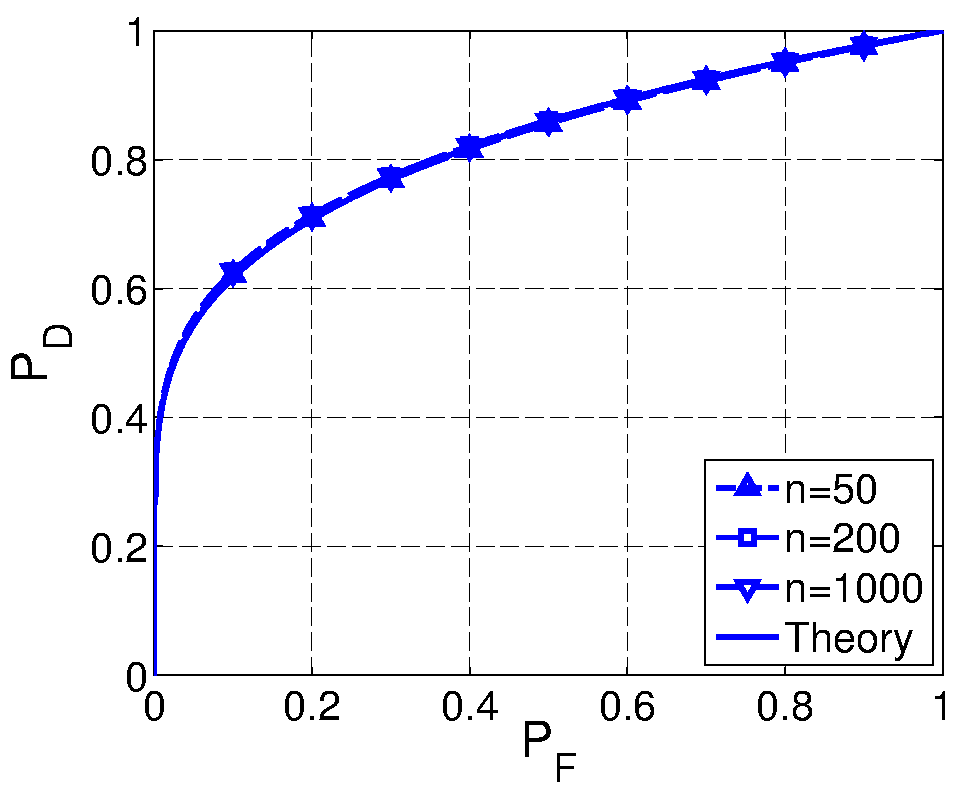
\includegraphics[width=1.5in]{figures/stoch_n_effect1.pdf}
\label{fig:stoch_n_effect1}
}
%\subfigure[$k=2$, $c=10$]{
%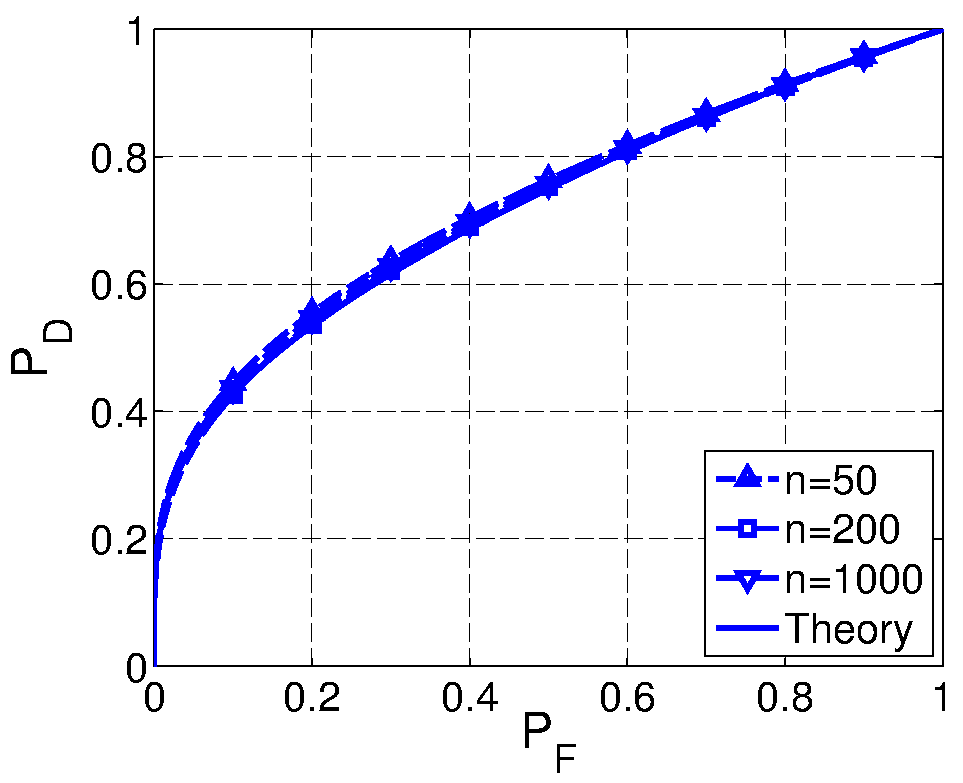
\includegraphics[width=3in]{figures/stoch_n_effect2.pdf}
%\label{fig:stoch_n_effect2}
%}
%\subfigure[$k=4$, $c=1$]{
%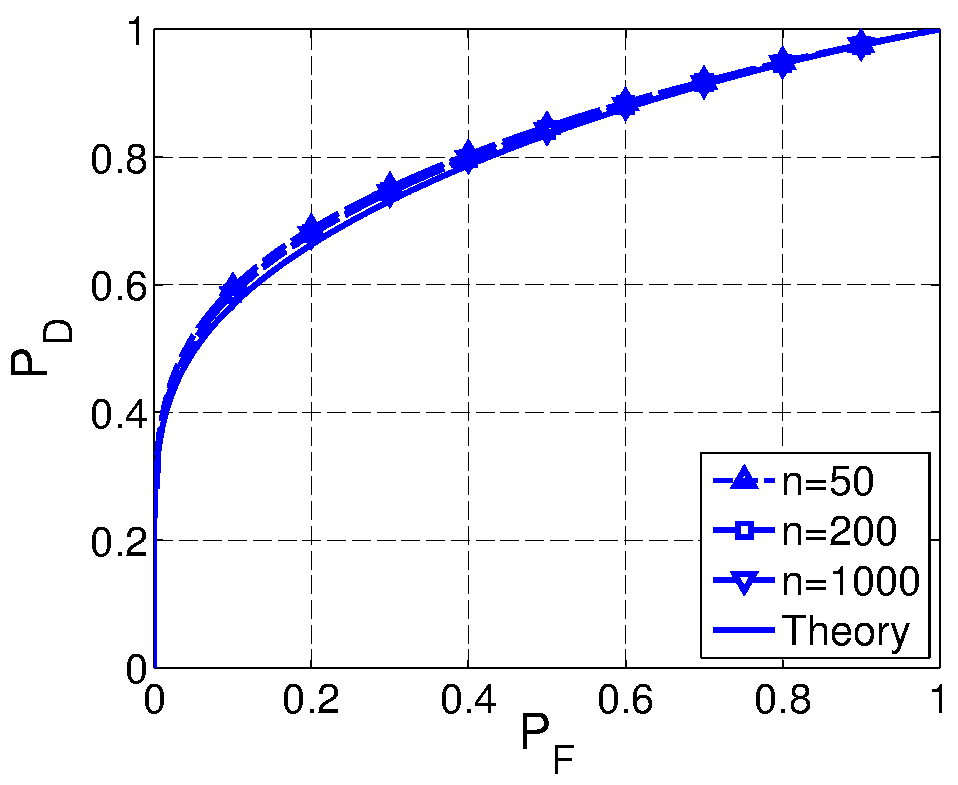
\includegraphics[width=3in]{figures/stoch_n_effect3.pdf}
%\label{fig:stoch_n_effect3}
%}
\subfigure[$k=4$, $c=10$]{
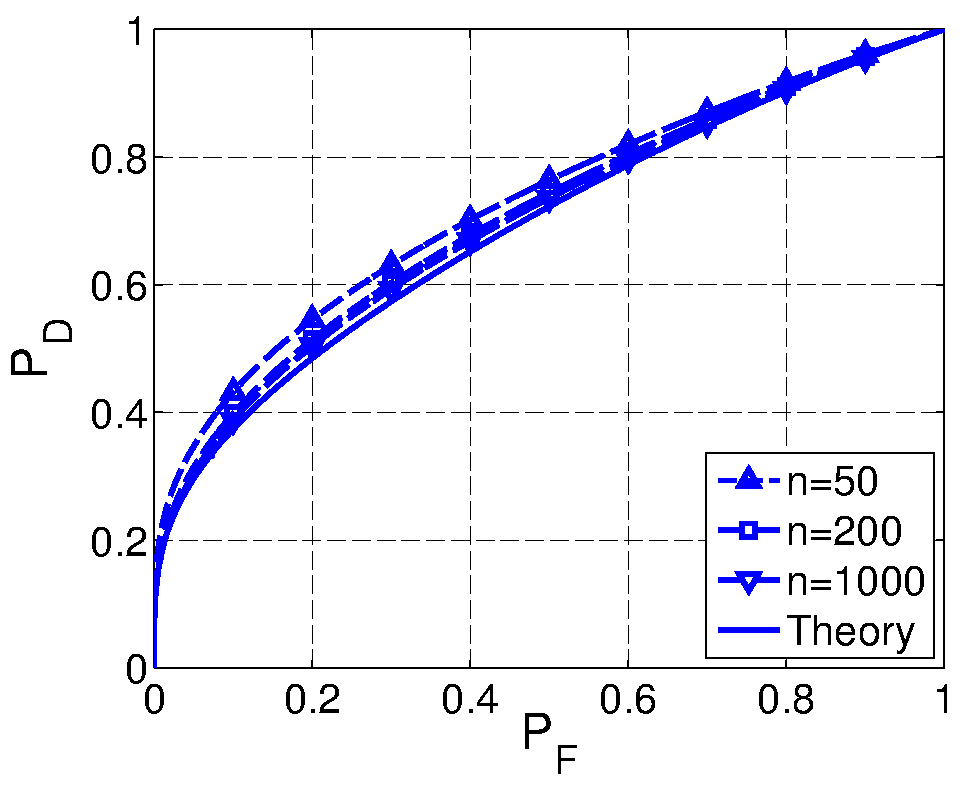
\includegraphics[width=1.5in]{figures/stoch_n_effect4.pdf}
\label{fig:stoch_n_effect4}
}
\vspace{-0.1in}
\caption{Empirical and theoretical ROC curves for the stochastic plug-in detector. Empirical ROC curves were simulated using $10000$ test samples and averaged over 50 trials using algorithms 2 and 4 of \cite{fawcett2006introduction}. (a) $\Sigma=\diag(10,2)$, $c=1$, $\widehat{k}=k=2$ so that $\keff=2$. (b) $\Sigma=\diag(10,2,0.5,0.1)$, $c=10$, $\widehat{k}=k=4$ so that $\keff=1$. Each figure plots empirical ROC curves for $n=50,200,1000$. Theoretical ROC curves were computed as described in Section \ref{sec:roc_theory}. As $n$ increases, the empirical ROC curves approach the theoretically predicted one. However, this convergence is slower for larger $k$ and $c$.}
\vspace{-0.3in}
\end{figure}

\textcolor{blue}{The theoretical ROC curve predictions for the plug-in and RMT detectors rely on the asymptotic approximations that ignore finite $n$ and $m$ correction terms. To examine the validity of the asymptotic approximations (Propositions \ref{th:angles} and \ref{th:eigvals_rmt}, Theorem \ref{th:other angles}, and Corollary \ref{corr:matrix}) and the rate of convergence, we consider two different settings for the stochastic plug-in detector. Figures \ref{fig:stoch_n_effect1}-\ref{fig:stoch_n_effect4} plot three empirical ROC curves for $n=50,200,1000$ as well as the theoretically predicted plug-in ROC curve. Each figure uses different values of $k$ and $c$ but in each case, $\widehat{k}=k$.}

\textcolor{blue}{For both figures, as $n$ increases, the empirical ROC curves approach the theoretical prediction, attesting to the asymptotic convergence of the RMT approximations. Analyzing the rate of convergence (which we conjecture to be $n^{1/2}$ for fixed $k$ and $c$) is an important open problem that we shall tackle in future work. As evident in Figures \ref{fig:stoch_n_effect1}-\ref{fig:stoch_n_effect4} the values of $k$ and $c$ play an important roll in the convergence of the empirical ROC curves. For the larger value of $k$ and $c$ (corresponding to the sample starved regime where the amount of training data is smaller than the system dimensionality i.e. $n>m$) the convergence is also slower. We see that for larger $k$ and $c$, when $n$ is small the empirical ROC curve is not well approximated by the asymptotic theoretical predictions. However, as $n$ increases, the deviation of the empircally generated ROC curve from the theoretically predicted one decreases. Claim \ref{th:other angles} suggests that the off diagonal terms of $\widehat{U}^HU$ asymptotically tend to zero. However, in the finite $n$ and $m$ case these terms are $O(1/\sqrt{n})$ and thus not identically zero. For larger rank systems (increased $k$), there are more of these non-identically-zero terms that worsen the approximation quality for fixed, relatively small $n$. As $n$ increases, this bias vanishes.}

\begin{figure}
\centering
\subfigure[Stochastic]{
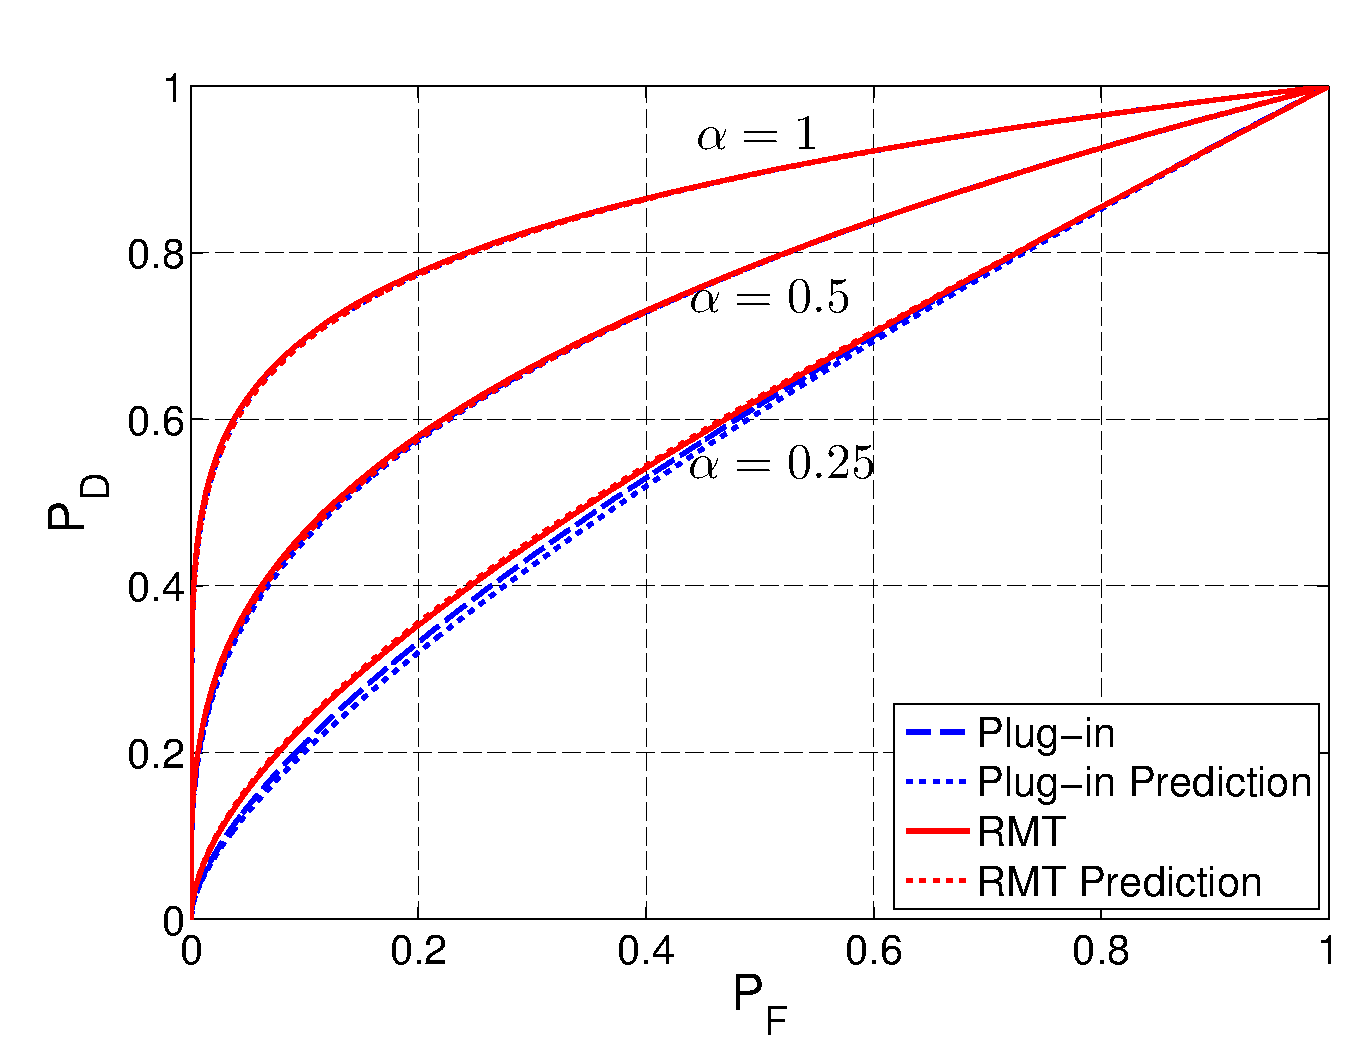
\includegraphics[width=1.5in]{figures/stoch_roc_pred.pdf}
\label{fig:stoch_roc_pred}
}
\subfigure[Deterministic]{
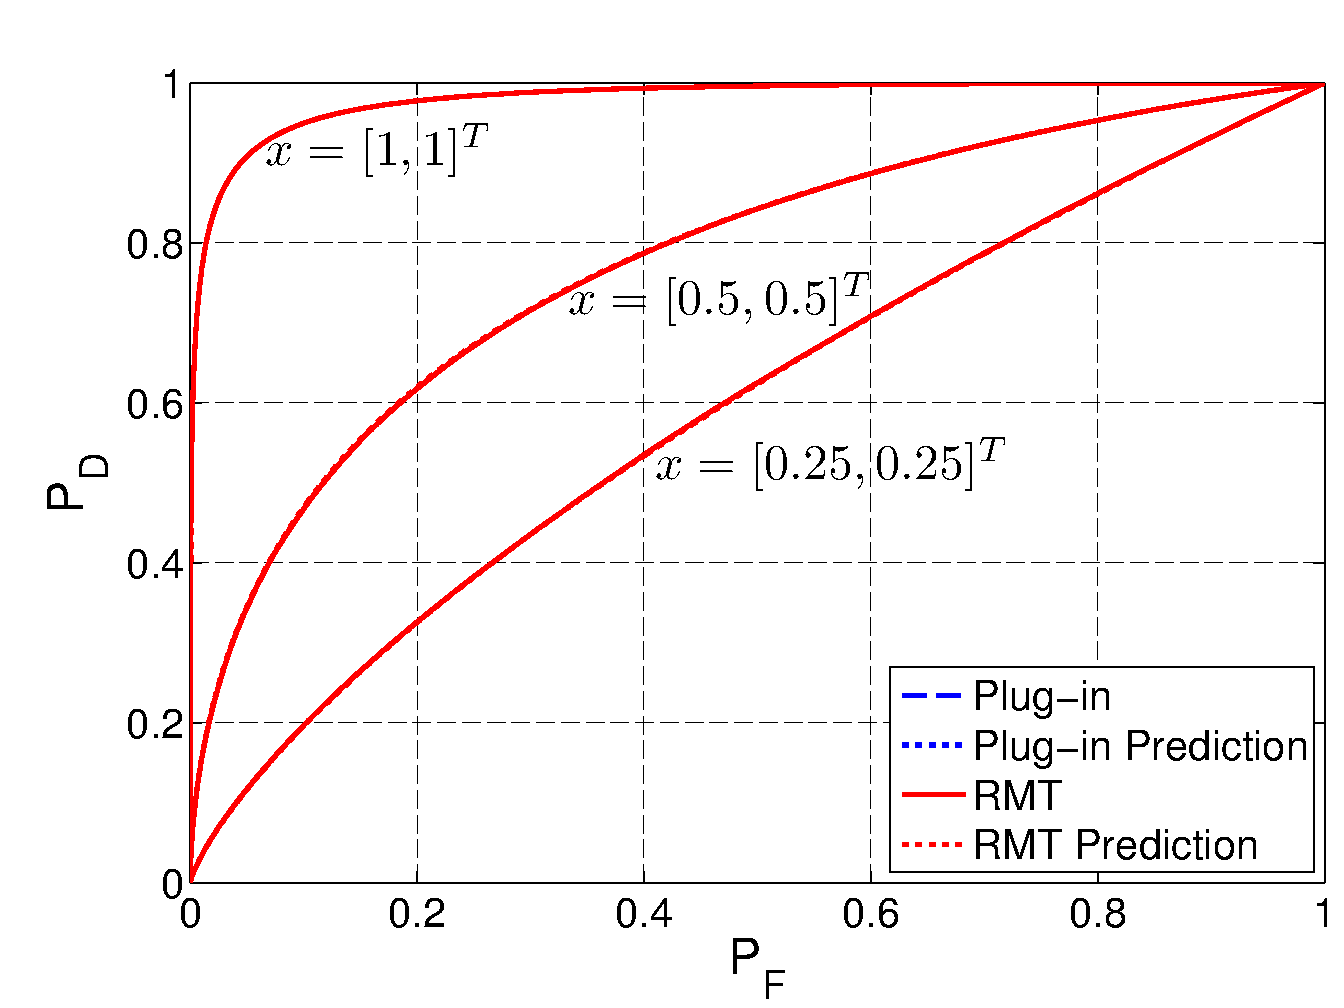
\includegraphics[width=1.5in]{figures/determ_roc_pred.pdf}
\label{fig:determ_roc_pred}
}
\vspace{-0.1in}
\caption{Empirical and theoretical ROC curves for the plug-in and RMT detectors. Empirical ROC curves were simulated using $10000$ test vectors and averaged over 100 trials with $n=1000$, $m=500$, and $\Sigma =\alpha\diag\left(10,5\right)$. The theoretical ROC curves were computed as described in Section \ref{sec:roc_theory}. (a) Stochastic testing seting. Results are plotted for $\alpha=1,0.5,0.25$. For $\alpha=1$ and $\alpha=0.5$, $\widehat{k}=k=k_\text{eff}=2$ by (\ref{eq:keff}). For $\alpha=0.25$, $k_\text{eff}=1$.Since $\widehat{k} > k_{\text{eff}}$ when $\alpha=0.25$, we observe a performance gain when using the RMT detector. (b) Deterministic testing setting. Results are plotted for $\alpha=1$ so that $\keff=2$. Three values of the deterministic signal vector were used: $x=[1,1]^T$, $x=[0.5,0.5]^T$, and $x=[0.25,0.25]^T$. The resulting ROC curves depend on the choice of $x$, however, since $\widehat{k} = k_{\text{eff}}$, the plug-in and RMT detector achieve the same performance for all $x$. For both the stochastic and deterministic detectors, the theoretically predicted ROC curves match the emprical ROC curves, reflecting the accuracy of Corollary \ref{corr:matrix} and the Lugannani-Rice formula.}
\vspace{-0.3in}
\end{figure}

The ROC predictions developed in Section \ref{sec:roc_theory} also depend on parameters such as $\Sigma$ and the deterministic vector $x$. To test the accuracy of the ROC predictions with respect to these parameters, we consider a setting where $\widehat{k}=k = 2$. Figure \ref{fig:stoch_roc_pred} plots empirical and theoretical ROC curves for the plug-in and RMT stochastic detectors for $\Sigma=\alpha\diag(10,5)$ for three choices of $\alpha$. As intuition suggests, smaller values of $\Sigma$ decrease the performance for both the plug-in and RMT detectors. For each choice of $\alpha$, the empirical ROC curves match the ROC predictions that rely on random matrix theoretic approximations presented in Section \ref{sec:rmt}. Using $\alpha=1$ or $\alpha=0.5$ results in $\keff=k=\widehat{k}=2$ but using $\alpha=0.25$ results in $k_\text{eff}=1$. As $\widehat{k}>k_\text{eff}$ for this last case, the plug-in detector realizes a performance loss compared to the RMT detector.

In the deterministic setting, $x$ is an additional parameter that affects detector performance. Figure \ref{fig:determ_roc_pred} plots empirical and theoretical ROC curves for the plug-in and RMT deterministic detectors for $\Sigma=\diag(10,5)$ for three choices of the deterministic test vector $x$. Larger values of $|x|$ result in better detector performance but for each choice of $x$, the theoretically predicted ROC curves match their empirical counterparts. As $x$ does not affect the value of $k_\text{eff}=\widehat{k}=k=2$, the plug-in and RMT detectors achieve the same performance because they have identical statistics. For both test vector models, the theoretical ROC curves match the empirical ROC curves thereby validating the accuracy of the random matrix theoretic approximations employed and the accuracy of the saddlepoint approximation to the c.d.f. used in the stochastic derivation. 

\subsection{Effect of the Number of Training Samples}

\begin{figure}
\centering
\subfigure[$m=5000$]{
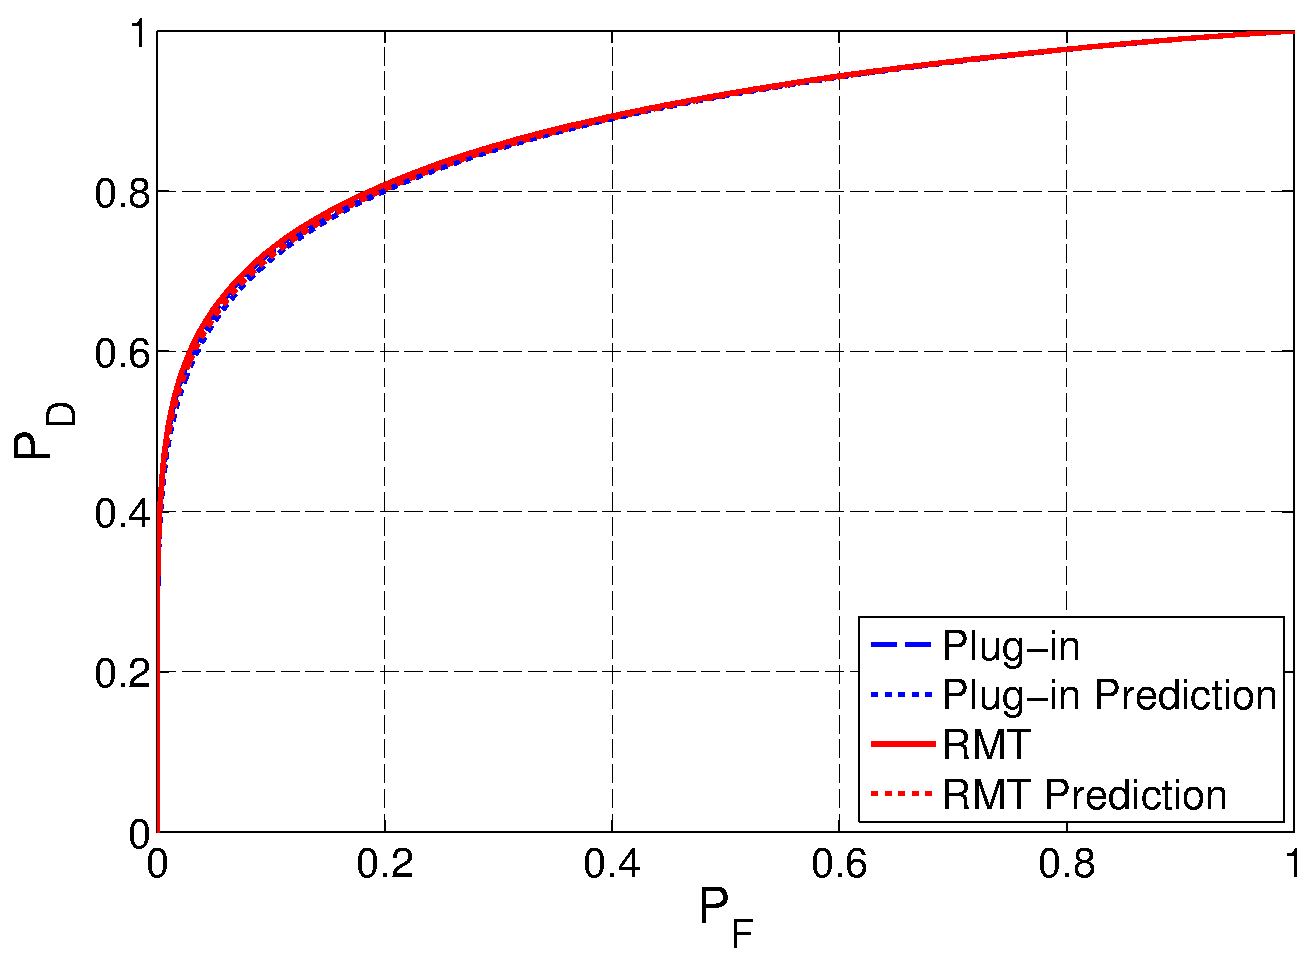
\includegraphics[width=1.5in]{figures/stoch_m_large.pdf}
\label{fig:stoch_m_large}
}
\subfigure[$m=250$]{
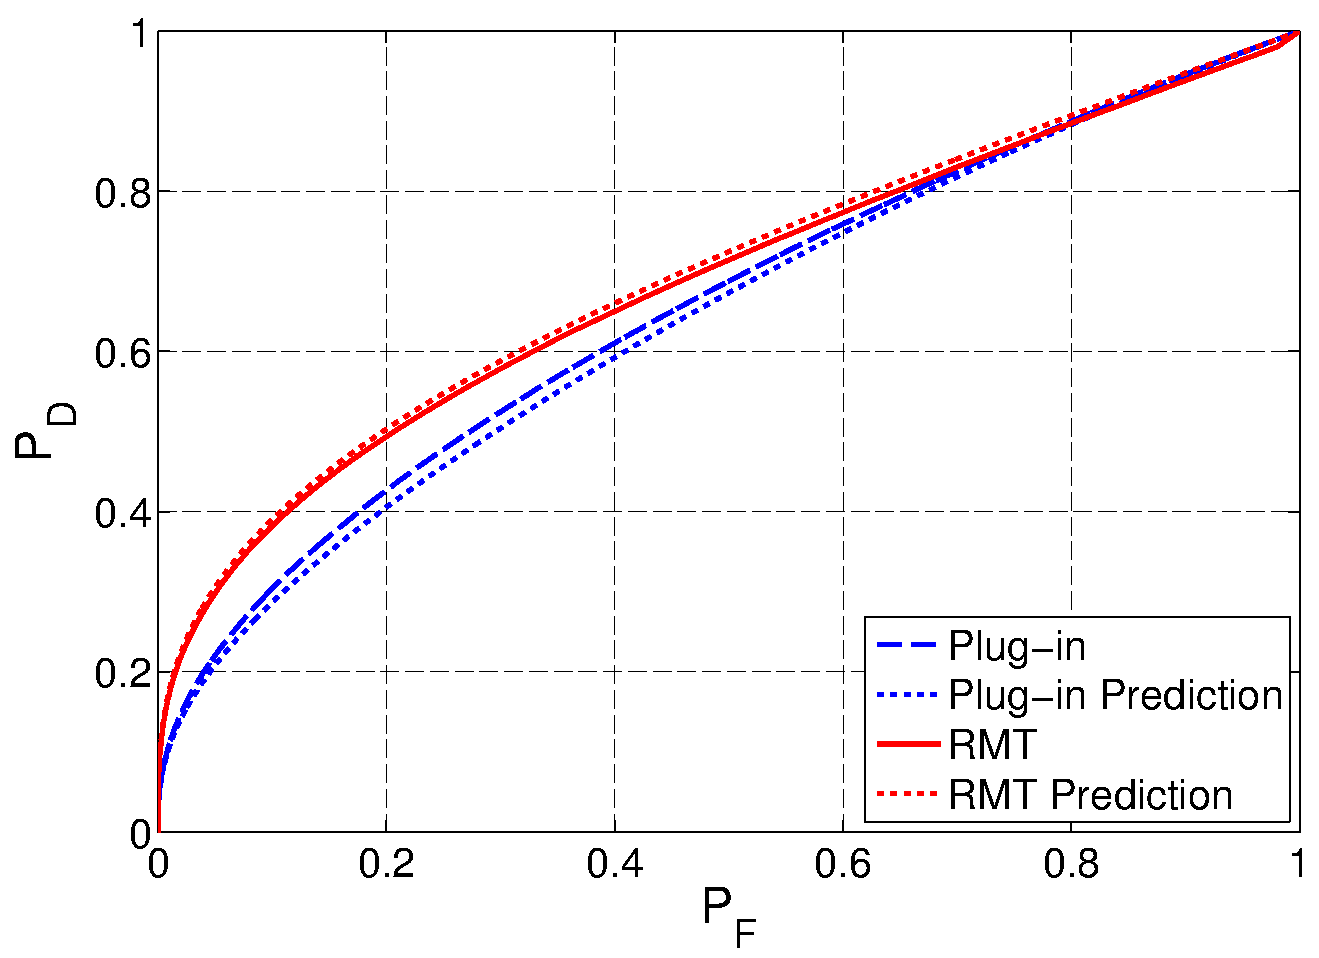
\includegraphics[width=1.5in]{figures/stoch_m_small.pdf}
\label{fig:stoch_m_small}
}
\vspace{-0.1in}
\caption{Empirical and theoretical ROC curves for the plug-in and RMT stochastic detectors. Empirical ROC curves were computed with 10000 test samples and averaged over 100 trials. Here, $n=5000$, $\widehat{k}=k=4$ and $\Sigma = \diag({\bf{10,3,2.5,2}})$. The empirical oracle ROC curve is provided for relative comparison purposes. (a) $m=5000$ so that $c=1$ and $k_\text{eff}=\widehat{k}=4$. The plug-in and RMT detectors achieve relatively the same performance. (b) $m=250$ so that $c=20$ and $\keff=1<\widehat{k}=4$. The RMT detector avoids some of the performance loss realized by the plug-in detector. As seen in Section \ref{sec:std_detecs}, limited training samples degrades detector performance. However, the new RMT detector does not suffer as badly as the plug-in detector because it accounts for subspace estimation errors due to finite training data. The disagreement between the theoretical and empirical ROC curves is attributed to finite dimensionality.}
\label{fig:stoch_m_effect}
\vspace{-0.3in}
\end{figure}

\textcolor{blue}{We saw in Section \ref{sec:training_effect} that finite training data degraded the performance of the plug-in detector relative to that of the oracle detector. The analysis of Section \ref{sec:rmt} mathematically justifies this observation showing that, for a fixed $\Sigma$, the number of training samples, $m$, directly affects $k_\text{eff}$ via (\ref{eq:keff}). While the plug-in detector ignores this analysis, we derived a new RMT detector that accounts for subspace estimation errors due to finite training data. By only using the $\keff$ informative signal subspace components, we hope that the RMT detector will avoid some of the performance loss associated with the plug-in detector. To explore how the number of training samples affects the relative performances of the plug-in and RMT detectors, we first consider the setting where $\widehat{k}=k=4$ with $\Sigma=\diag(10,3,2.5,2)$. }

Figures \ref{fig:stoch_m_large} and \ref{fig:determ_m_large} investigate the performance when $m=n$ so that $c=1$ for the stochastic and deterministic settings, respectively. This choice of $m$ results in $k_\text{eff}=\widehat{k}=4$. As expected, for both settings the plug-in and RMT detectors achieve relatively the same performance because $\widehat{k}=\keff$. Figures \ref{fig:stoch_m_small} and \ref{fig:determ_m_small} choose $20m=n$ so that $c=20$ and $k_\text{eff}=1$ for the stochastic and deterministic settings, respectively. This corresponds to the sample starved regime where $m<n$. In this second experiment, the plug-in detectors becomes suboptimal for both testing settings because they use $4=\widehat{k} > k_\text{eff}=1$ subspace components. Whenever $k_\text{eff}<\widehat{k}$ the RMT detectors avoid some of the performance loss (compared to the oracle detectors) realized by the plug-in detectors. We could have observed this same effect by instead varying $\Sigma$ as both of these quantities drive the value of $k_\text{eff}$. The disagreement between the theoretical and empirical stochastic ROC curves for the plug-in detector is attributed to the finite $n$ and $m$ correction terms, which we have discussed previously.

\textcolor{blue}{Figures \ref{fig:stoch_m_effect} and \ref{fig:determ_m_effect} show that the number of training samples helps to drive the performance of matched subspace detectors. In Section \ref{sec:std_detecs}, we mathematically defined the performance loss of a detector relative to its oracle detector as $\epsilon$ in (\ref{eq:epsilon}) and empirically plotted the number of training samples needed to achieve a desired performance loss for the stochastic plug-in detector in Figure \ref{fig:epsilon_graph}. Figures \ref{fig:stoch_theory_epsilon} and \ref{fig:determ_theory_epsilon} theoretically plot this same curve for the plug-in and RMT detectors for each testing setting, respectively.}

\textcolor{blue}{These figures show that when $\keff<\widehat{k}$, the RMT detector achieves a much smaller performance loss for a fixed number of training samples. Put another way, to achieve the same performance loss, the RMT detectors need a significantly less number of training samples when $\keff<\widehat{k}$. Figure \ref{fig:stoch_theory_epsilon} shows that the stochastic detectors can acheive an arbitrarily small performance loss given a particularly large number of training samples. However, Figure \ref{fig:determ_theory_epsilon} shows that there is a performance loss limit for the deterministic detectors and that this limit may be different for the RMT and plug-in detectors. As discussed in Section \ref{sec:std_detecs}, this arises because the oracle deterministic detector assumes that $x$ is known. As $m\to\infty$, $\widehat{U}\to U$ and $\widehat{\Sigma}\to\Sigma$, however, the plug-in detector's estimate of $\widehat{x}$ still depends on the noisy observed data $y$. Therefore, unlike the stochastic detectors that can achieve an arbitrarily small performance loss, the deterministic plug-in and RMT detectors can never achieve the same performance as the deterministic oracle detector.}

\begin{figure}
\centering
\subfigure[$m=5000$]{
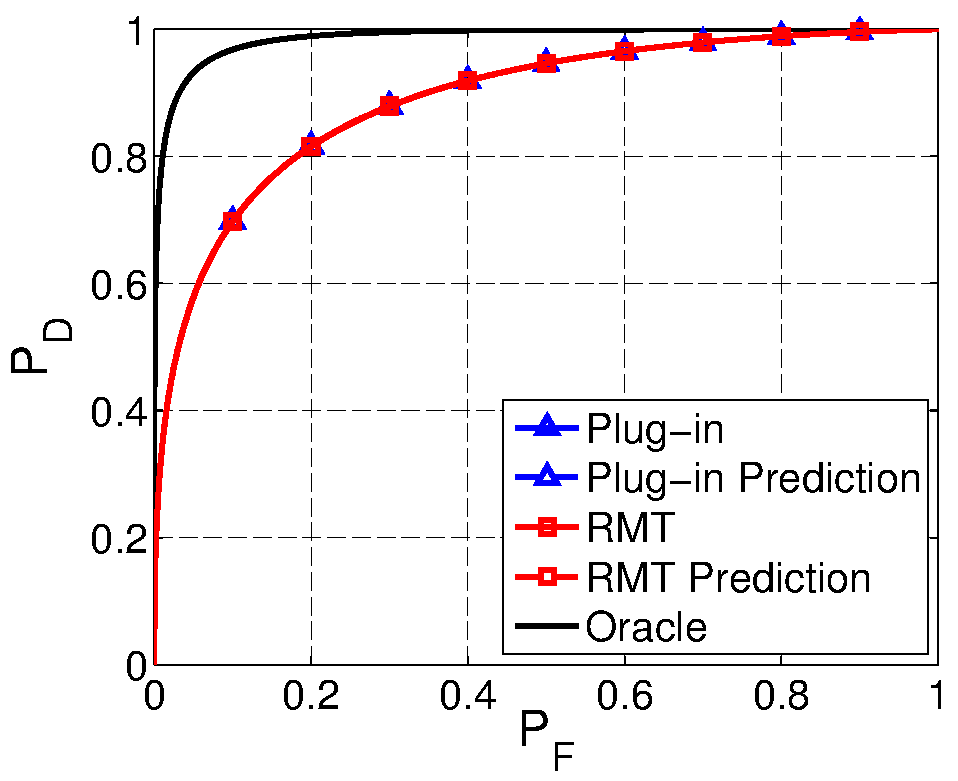
\includegraphics[width=1.5in]{figures/determ_m_large.pdf}
\label{fig:determ_m_large}
}
\subfigure[$m=250$]{
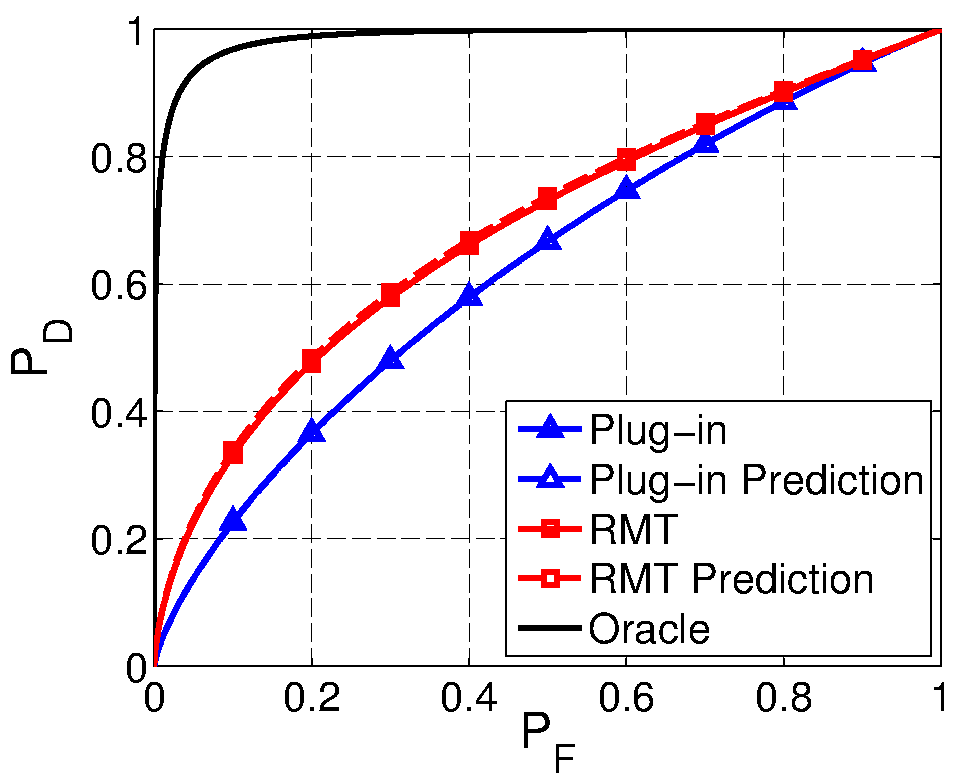
\includegraphics[width=1.5in]{figures/determ_m_small.pdf}
\label{fig:determ_m_small}
}
\vspace{-0.1in}
\caption{Analagous figures to Figures \ref{fig:stoch_m_large} and \ref{fig:stoch_m_small} for the deterministic detectors when $x=0.75\times[1,1,1,1]^T$. When $\keff<\widehat{k}$ we see that the RMT detector avoids some of the performance loss of the plug-in detector due to finite training data.}
\label{fig:determ_m_effect}
\vspace{-0.2in}
\end{figure}

\begin{figure}
\centering
\subfigure[Stochastic]{
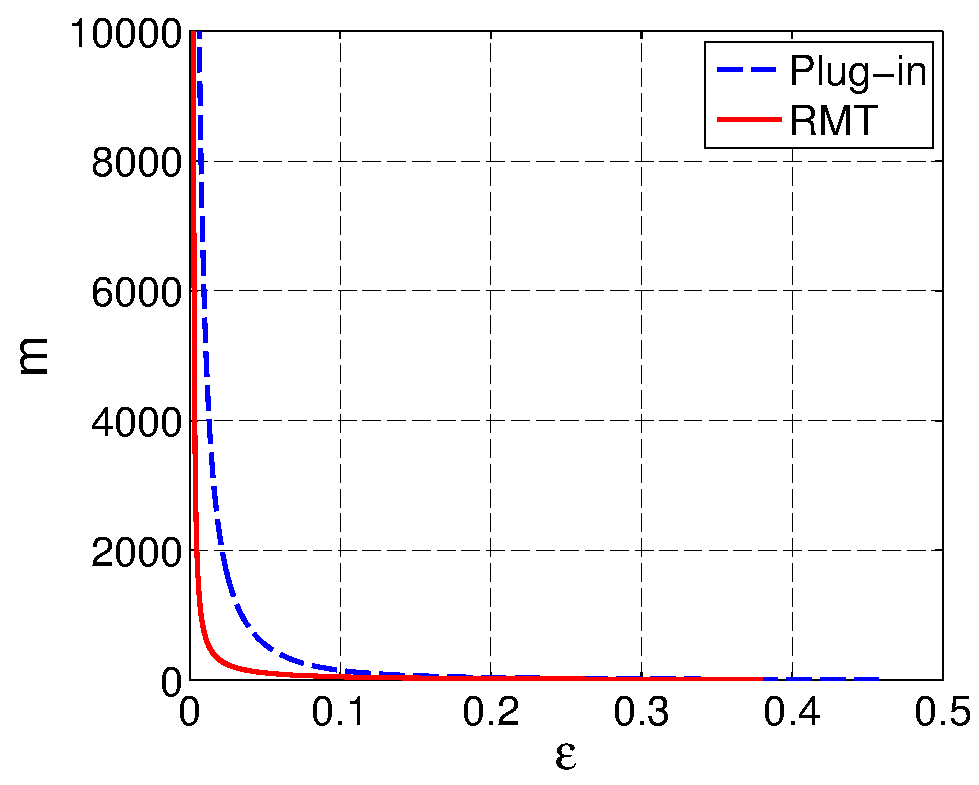
\includegraphics[width=1.5in]{figures/stoch_theory_epsilon_graph.pdf}
\label{fig:stoch_theory_epsilon}
}
\subfigure[Deterministic]{
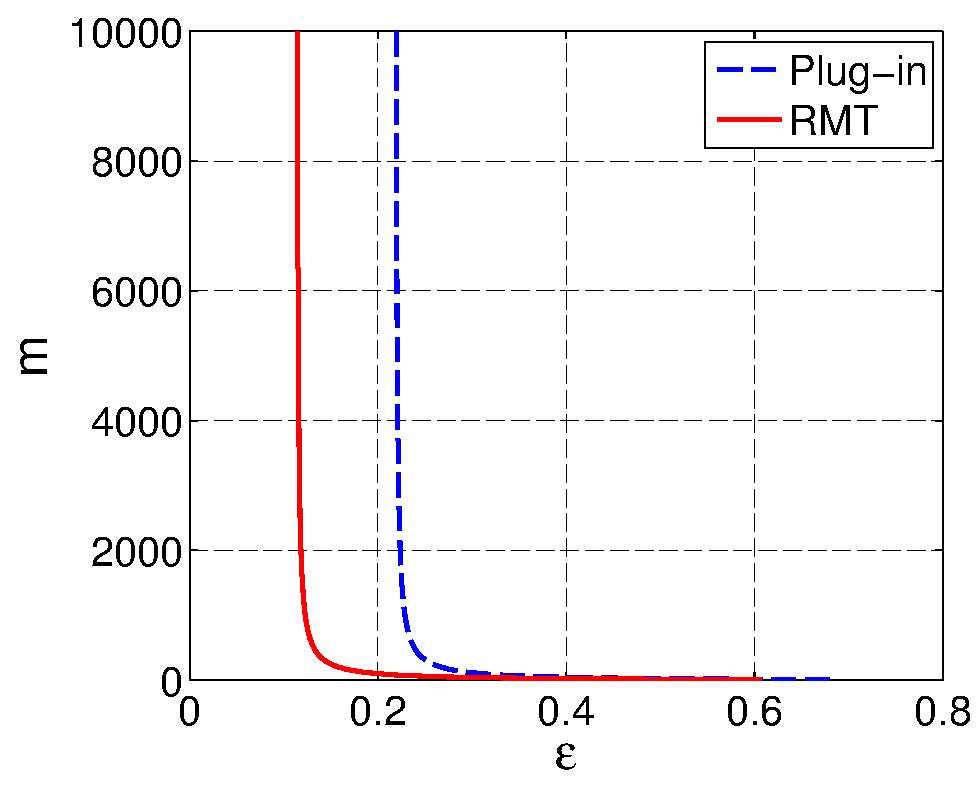
\includegraphics[width=1.5in]{figures/determ_theory_epsilon_graph.pdf}
\label{fig:determ_theory_epsilon}
}
\vspace{-0.1in}
\caption{Theoretically determined number of training samples, $m$, needed to achieve a desired performance loss, $\epsilon$, as defined in (\ref{eq:epsilon}). The required false alarm rate is $P_F=0.1$ with $n=200$, $\Sigma = \diag(10,0.1)$, and $\widehat{k}=k=2$. (a) Results for the stochastic detectors. We see that for a given $\epsilon$, the new RMT detector requires less training samples. (b) Results for the deterministic detectors when $x=[0.75,0.75]^T$. Again, for a given $\epsilon$, the new RMT detector requires less training samples. In the deterministic setting, the limiting performance loss is different (and non-zero) for the plug-in and RMT detectors. This arises in estimation errors of $x$ in the GLRT.}
\label{fig:epsilon_combined}
\end{figure}


%we have neglected. As $k$ increases, there are more off-diagonal terms in the covariance matrix in (\ref{eq:cov mat}) that are not identically zero, as discussed earlier. Theorem \ref{th:other angles} shows that asymptotically these off diagonal terms decay to zero but in the finite $n$ and $m$ case, they are non-zero. In the case of larger $k$, there are more of these non-identically-zero terms thereby worsening the approximation.

\subsection{Effect of $\widehat{k}$}
\begin{figure}
\centering
\subfigure[Stochastic]{
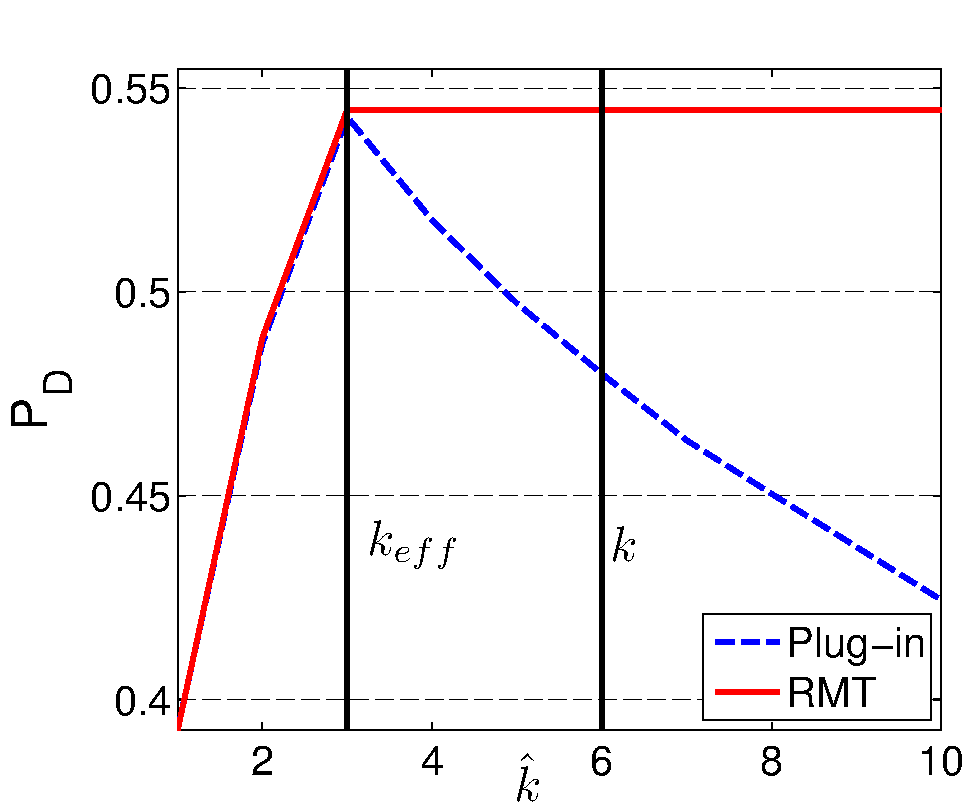
\includegraphics[width=1.5in]{figures/stoch_khat_graph.pdf}
\label{fig:stoch_khat}
}
\subfigure[Deterministic]{
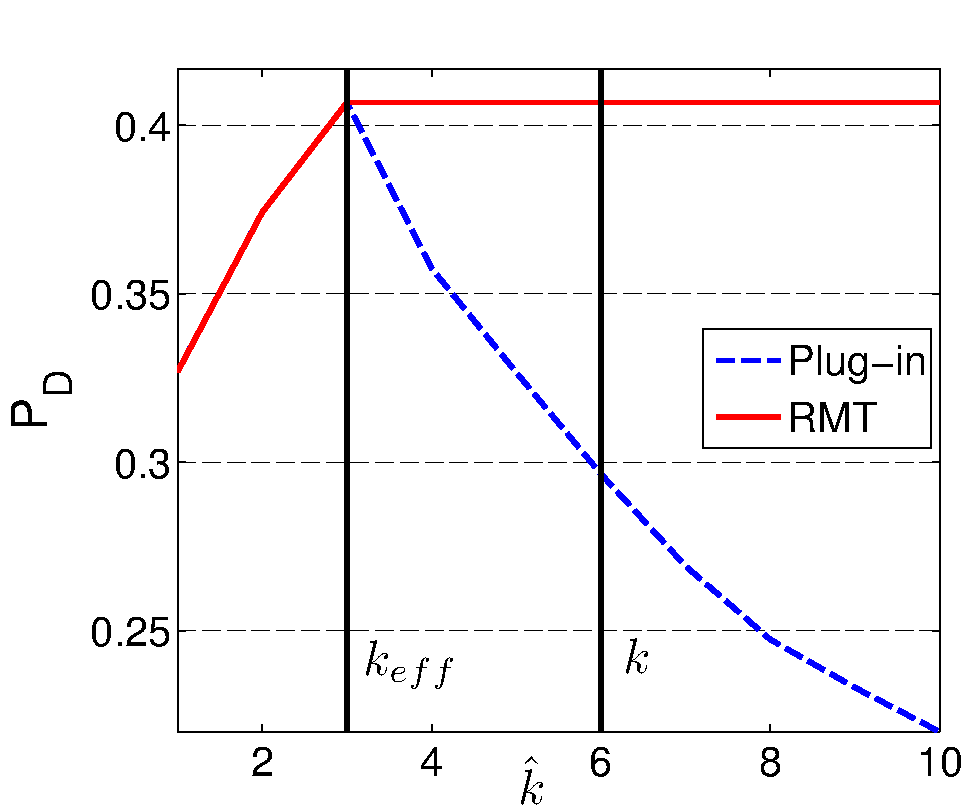
\includegraphics[width=1.5in]{figures/determ_khat_graph.pdf}
\label{fig:determ_khat}
}
\vspace{-0.1in}
\caption{Empirical exploration of the achieved probability of detection, $P_D$, for a fixed probability of false alarm, $P_F=0.01$, for various $\widehat{k}$. Empirical ROC curves were computed using 10000 test samples and averaged over 100 trials with $n=1000$, $m=500$, and $\Sigma = \diag({\bf{10,5,4}},0.75,0.5,0.25)$ so that $k_{\text{eff}}=3$. (a) Results for the stochastic detectors. (b) Results for the deterministic detecotrs using $x=0.75\times[1,1,1,1,1,1]^T$. In both test settings, the optimal $\widehat{k}$ resulting in the largest $P_D$ is not the true $k$, but rather $k_\text{eff}$.}
\label{fig:khat_graphs}
\vspace{-0.3in}
\end{figure}

\textcolor{blue}{We discussed in Section \ref{sec:param_estim} that we are given a dimension estimate $\widehat{k}$ when deriving our detector. From our perspective, we don't know how $\widehat{k}$ was estimated (possibly from the training data or by a domain expert) but simply use it when forming our subpsace and signal covariance estimates.} Figures \ref{fig:stoch_khat} and \ref{fig:determ_khat} empirically examine the performance of the plug-in and RMT detectors as a function of $\widehat{k}$ for the stochastic and deterministic test settings, respectively. Here, we relax the constraint that $\widehat{k}\geq k$. The figures plot the achieved probability of detection for a constant false alarm rate of $0.01$. The result confirms that, for both settings, $k_\text{eff}$ is the optimal choice for $\widehat{k}$. When the plug-in detectors use $\widehat{k} = k_\text{eff}$ they achieve an equivalent performance as that of the RMT detector.

Setting $\widehat{k} < \keff$ drastically degrades performance for all detectors. In this regime, the plug-in and RMT detectors realize the same ROC performance, demonstrating that quantification and exploitation of the subspace estimation accuracy ($|\langle u_i,\widehat{u}_i\rangle |^2_{\text{rmt}}$ and $\sigma_{i_\text{rmt}}^2$), while useful in ROC performance prediction, does \textit{not} noticeably enhance detection performance. When $\widehat{k} > k_\text{eff}$, the performances of the plug-in detectors degrade while those of the RMT detectors are stable as if $\widehat{k}=k_\text{eff}$. In other words, we do not pay a price for overestimating the subspace dimension with the RMT detectors. This makes sense (and is slightly contrived) because the RMT detectors will only sum to a maximum of $k_\text{eff}$ indices as evident in (\ref{eq:optimal_stat_stoch}) and (\ref{eq:optimal_stat_determ}). In many applications, practitioners might employ the ``play-it-safe'' approach and set $\widehat{k}$ to be significantly greater than $k_\text{eff}$. The performance loss caused by adding each uninformative subspace, as seen in Figure \ref{fig:khat_graphs}, constitutes evidence to the assertion that overestimating the signal subspace dimension is a bad idea. When $k_\text{eff} < k$, even perfectly estimating the subspace dimension (i.e. setting $\widehat{k} = k$) is suboptimal.


\section{Conclusion}\label{sec:conclusion}
In this paper, we considered a matched subspace detection problem where the low-rank signal subspace is unknown and must be estimated from finite, noisy, signal-bearing training data. We considered both a stochastic and deterministic model for the testing data. The subspace estimate is inaccurate due to finite and noisy training samples and therefore degrades the performance of plug-in detectors compared to an oracle detector. We showed how the ROC performance curve can be derived from the RMT-aided quantification of the subspace estimation accuracy.

Armed with this RMT knowledge, we derived a new RMT detector that only uses the effective number of informative subspace components, $k_\text{eff}$. Plug-in detectors that use the uninformative components will thus incur a performance degradation, relative to the RMT detector. \textcolor{blue}{In settings where a practitioner might play-it-safe and set $\widehat{k}> \widehat{k}_{\text{eff}}$, the performance loss in significant (see Figures \ref{fig:stoch_theory_epsilon} and \ref{fig:determ_theory_epsilon} for a demonstration of how much training data such a play-it-safe plug-in detector would need to match the performance of a $\keff$-tuned RMT detector).} This highlights the importance of robust techniques \cite{nadakuditi2010fundamental,johnstone2001distribution,el2007tracy} for estimating $k_\text{eff}$ in subspace based detection schemes as opposed to estimating $k$, particularly in the regime where $k_{\text{eff}} < k$.  We showed in Tables \ref{table:summary_stoch} and \ref{table:summary_determ} that the distributions of the test statistics could be expressed as a weighted sum of independent chi-squared random variables. The associated ROC curves can then be computed using a saddlepoint approximation.

\textcolor{blue}{The results in this paper can be extended in several directions. We note that the stochastic detector setting assumed normally distributed training and test data. We can extend the analysis to the Gaussian training data but non-Gaussian test vector setting by `integrating-out' the deterministic detector performance curves with respect to the non-Gaussian distribution of the test-vector. Our results relied on characterization of the quantity $\langle u_{j},\widehat{u}_{i}\rangle$.  Thus analogous performance curves can be obtained for any alternate training data models for which this quantity can be analytically quantified. To that end, the results in \cite{benaych2011singular} facilitate such an analysis for a broader class of models including the correlatted Gaussians training data setting. An extension to the missing data setting might follow a similar approach and appears within reach. Aspects related to rate of convergence are open and will be the subject of future work.}



\section*{Appendix}
\textit{Theorem 5.1:} Assume the same hypothesis as in Proposition \ref{th:angles}. Let $\widehat{k}=\keff=k$. For $i=1,\dots,\widehat{k}$, $j=1,\dots,k$, and $i\neq j$, as $n,m\to\infty$ with $n/m\to c$, then $\langle u_j,\widehat{u}_i\rangle \convas 0.$
\begin{proof}
Let $U_{n,k}$ be a $n\times k$ real or complex matrix with orthonormal columns, $u_i$ for $1\leq i\leq k$. Let $\Sigma = \diag\left(\sigma_1^2,\dots,\sigma_k^2\right)$ such that $\sigma_1^2>\sigma_2^2>\dots>\sigma_k^2>0$ for $k\geq 1$. Define $P_n=U_{n,k}\Sigma U_{n,k}^H$ so that $P_n$ is rank-$k$. Let $Z_n$ be a $n\times m$ real or complex matrix with independent $\mathcal{CN}\left(0,1\right)$ entries. Let $X_n=\frac{1}{m}Z_nZ_n^H$, which is a random Wishart matrix, have eigenvalues $\lambda_1(X_n)\geq\dots\geq\lambda_n(X_n)$. Let $\widehat{X}_n=X_n\left(I_n+P_n\right)$. $X_n$ and $P_n$ are independent by assumption. Define the empirical eigenvalue distribution as $\mu_{X_n}=\frac{1}{n}\sum_{j=1}^n\delta_{\lambda_j\left(X_n\right)}$. We assume that as $n\to\infty$, $\mu_{X_n}\overset{\text{a.s.}}{\longrightarrow}\mu_X$.


For $i=1,\dots, \widehat{k}=k$, let $\widehat{v}_i$ be an arbitrary unit eigenvector of $\widehat{X}_n$. By the eigenvalue master equation, $\widehat{X}_n\widehat{v}_i=\widehat{\lambda}_i\widehat{v}_i$, it follows that
\begin{equation}\label{eq:eval_master}
\begin{aligned}
  &U_{n,k}^H\left(\widehat{\lambda}_iI_n-X_n\right)^{-1}X_nU_{n,k}\Sigma U_{n,k}^H\widehat{v}_i&&=U_{n,k}^H\widehat{v}_i.\\
\end{aligned}
\end{equation}
Let $X_n=V_n\Lambda_nV_n^H$ be the eigenvalue decomposition of $X_n$ such that $\Lambda_n=\diag(\lambda_1(X_n),\dots,\lambda_n(X_n))$ and $\lambda_1(X_n)\geq\dots\geq\lambda_n(X_n)$. Using this decomposition and defining $W_{n,k}=V^HU_{n,k}$, (\ref{eq:eval_master}) simplifies to
\begin{equation}\label{eq:eval_master2}
\begin{aligned}
  &W_{n,k}^H\left(\widehat{\lambda}_iI_n-\Lambda_n\right)^{-1}\Lambda_nW_{n,k}\Sigma U_{n,k}^H\widehat{v}_i&&=U_{n,k}^H\widehat{v}_i.\\
\end{aligned}
\end{equation}
Define the columns of $W_{n,k}$ to be $w_j^{(n)}=[w_{1,j}^{(n)},\dots,w_{n,j}^{(n)}]^T$ for $j=1,\dots,k$. These columns are orthonormal and isotropically random. We can rewrite (\ref{eq:eval_master2}) as
\begin{equation}\label{eq:t_trans}
\left[T_{\mu_{r,j}^{\left(n\right)}}\left(\widehat{\lambda}_i\right)\right]_{r,j=1}^k \Sigma U_{n,k}^H\widehat{v}_i=U_{n,k}^H\widehat{v}_i
\end{equation}
where for $r=1,\dots,k$, $j=1,\dots,k$, $\mu_{r,j}^{\left(n\right)}=\sum_{\ell=1}^n\overline{w_{\ell,r}^{\left(n\right)}}w_{\ell,j}^{\left(n\right)}\delta_{\lambda_\ell\left(X_n\right)}$ is a complex measure and $T_{\mu_{r,j}^{\left(n\right)}}$ is the T-transform defined by $T_{\mu}\left(z\right) = \int\frac{t}{z-t}d\mu\left(t\right)\,\,\,\,\text{for } z\not\in\text{supp } \mu$. We may rewrite (\ref{eq:t_trans}) as
\begin{equation*}
\left(I_k-\left[\sigma_j^2T_{\mu_{r,j}^{\left(n\right)}}\left(\widehat{\lambda}_i\right)\right]_{r,j=1}^k\right)U_{n,k}^H\widehat{v}_i=0.
\end{equation*}
Therefore, $U_{n,k}^H\widehat{v}_i$ must be in the kernel of $M_n\left(\widehat{\lambda}_i\right)=I_k-\left[\sigma_j^2T_{\mu_{r,j}^{\left(n\right)}}\left(\widehat{\lambda}_i\right)\right]_{r,j=1}^k$.
By Proposition 9.3 of \cite{benaych2011eigenvalues}
\begin{equation*}
\mu_{r,j}^{\left(n\right)}\overset{\text{a.s.}}{\longrightarrow}\begin{cases}\mu_X & \text{for } i=j \\ \delta_0 & \text{o.w.} \end{cases}
\end{equation*}
where $\mu_X$ is the limiting eigenvalue distribution of $X_n$. Therefore,
\begin{equation*}
M_n\left(\widehat{\lambda}_i\right)\overset{\text{a.s.}}{\longrightarrow}\diag\left(1-\sigma_1^2T_{\mu_X}\left(\widehat{\lambda}_i\right), \dots, 1-\sigma_k^2T_{\mu_X}\left(\widehat{\lambda}_i\right)\right).
\end{equation*}
As $k_\text{eff}=k$, for $i=1,\dots,k$, $\sigma_i^2>1/T_{\mu_X}(b^+)$, where $b$ is the supremum of the support of $\mu_X$. As $\widehat{\lambda}_i$ is the eigenvalue corresponding to the eigenvector $\widehat{v}_i$, by Theorem 2.6 of \cite{benaych2011eigenvalues} $\widehat{\lambda}_i\overset{\text{a.s.}}{\longrightarrow}T^{-1}_{\mu_X}\left(1/\sigma_i^2\right)$. Therefore,
\footnotesize\begin{equation}\label{eq:Mn}
M_n\left(\widehat{\lambda}_i\right)\overset{\text{a.s.}}{\longrightarrow}\diag\left(1-\frac{\sigma_1^2}{\sigma_i^2}, \dots, 1-\frac{\sigma_{i-1}^2}{\sigma_i^2}, 0, 1-\frac{\sigma_{i+1}^2}{\sigma_i^2}, \dots, 1-\frac{\sigma_k^2}{\sigma_i^2}\right)
\end{equation}\normalsize
Recall that $U_{n,k}^H\widehat{v}_i$ must be in the kernel of $M_n\left(\widehat{\lambda}_i\right)$. Therefore, any limit point of $U_{n,k}^H\widehat{v}_i$ is in the kernel of the matrix on the right hand side of (\ref{eq:Mn}). Therefore, for $i\neq j$, $i=1,\dots,\widehat{k}$, $j=1,\dots,k$, we must have that $\left(1-\frac{\sigma_j^2}{\sigma_i^2}\right)\langle u_j,\widehat{v}_i\rangle=0$. As $\sigma_i^2\neq\sigma_j^2$, for this condition to be satisfied we must have that for $j\neq i$, $i=1,\dots,\widehat{k}$, $j=1,\dots,k$, $\langle u_j,\widehat{v}_i\rangle\overset{\text{a.s.}}{\longrightarrow}0$.

Recall that our observed vectors $y_i\in\complex^{n\times 1}$ have covariance matrix $U_{n,k}\Sigma U_{n,k}^H+I_n=P_n+I_n$. Therefore, our observation matrix, $Y_n$ which is a $n\times m$ matrix, may be written $Y_n=\left(P_n+I_n\right)^{1/2}Z_n$. The sample covariance matrix, $S_n=\frac{1}{m}Y_nY_n^H$, may be written $S_n=\left(I_n+P_n\right)^{1/2}X_n\left(I_n+P_n\right)^{1/2}$. By similarity transform, if $\widehat{v}_i$ is a unit-norm eigenvector of $\widehat{X}_n$ then $\widehat{s}_i=\left(I_n+P_n\right)^{1/2}\widehat{v}_i$ is an eigenvector of $S_n$. If $\widehat{u}_i=\widehat{s}_i/\|\widehat{s}_i\|$ is a unit-norm eigenvector of $S_n$, it follows that
\begin{equation*}
\langle u_j,\widehat{u}_i\rangle=\frac{\sqrt{\sigma_i^2+1}\langle u_j,\widehat{v}_i\rangle}{\sqrt{\sigma_i^2|\langle u_j,\widehat{v}_i\rangle|^2+1}}
\end{equation*}
As $\langle u_j,\widehat{v}_i\rangle\overset{\text{a.s.}}{\longrightarrow}0$ for all $i\neq j$, $i=1,\dots,\widehat{k}$, $j=1,\dots,k$, it follows that $\langle u_j,\widehat{u}_i\rangle\overset{\text{a.s.}}{\longrightarrow}0$ for all $i\neq j$ $i=1,\dots,\widehat{k}$, $j=1,\dots,k$.

%%%%%%%%%%%%%%%%%%%%% CLAIM %%%%%%%%%%%%%%%%%%%%%%%%%%%%%%%%%%%%%%%%%%%%%

\textit{Claim 5.1:}  We conjecture that this result holds for the general case of $i\neq
j$, $i=1,\dots,\widehat{k}$, $j=1,\dots,k$, not just when $\widehat{k}=\keff=k$. Consider
the case when $k=1$. For $i>2$, if $\widehat{\lambda}_i$ is an eigenvalue of
$\widehat{X}_n=X_n(I_n+\sigma^2uu^H)$, then it satisfies
$\det(\widehat{\lambda}_iI_n-X_n(I_n+\sigma^2uu^H)) =
\det(\widehat{\lambda}_iI_n-X_n)\det(I_n-(\widehat{\lambda}_iI_n-X_n)^{-1}X_n\sigma^2uu^H)=0$. Therefore,
if $\widehat{\lambda}_i$ is not an eigenvalue of $X_n$, the corresponding unit norm
eigenvector $\widehat{v}_i$ is in the kernel of
$I_n-(\widehat{\lambda}_iI_n-X_n)^{-1}X_n\sigma^2uu^H$. Therefore
\begin{equation*}
  |\langle \widehat{v}_i,u\rangle |^2 = \frac{1}{\sigma^4u^HX_n\left(\widehat{\lambda}_iI_n-X_n\right)^{-2}X_nu}.
\end{equation*}
Recall that Weyl's interlacing lemma for eigenvalues gives $\lambda_i(X_n)\leq
\widehat{\lambda}_i\leq \lambda_{i-1}(X_n)$. Letting $X_n=V_n\Lambda_nV_n^H$ and
$w=V_n^Hu$, we see the importance of the
asymptotic spacing of eigenvalues of $X_n$ in
%\begin{equation*}
%  u^HX_n(\widehat{\lambda}_jI_n-X_n)^{-2}X_nu =\sum_{\ell=1}^n\frac{|w_\ell|^2\lambda_\ell^2(X_n)}{\left(\widehat{\lambda}_j-\lambda_\ell\right)^2}\geq\frac{|w_{j-1}|^2\lambda_{j-1}^2(X_n)}{|\lambda_{j-1}-\lambda_j|^2}+\frac{|w_{j}|^2\lambda_j^2(X_n)}{|\lambda_{j-1}-\lambda_j|^2}.
%\end{equation*}
\begin{equation*}
  u^HX_n(\widehat{\lambda}_iI_n-X_n)^{-2}X_nu
  =\sum_{\ell=1}^n\frac{|w_\ell|^2\lambda_\ell^2(X_n)}{\left(\widehat{\lambda}_i-\lambda_\ell\right)^2}\geq
  \frac{\min_j\lambda_j^2(X_n)\min_j|w_j|^2}{\max_j |\lambda_{j-1}-\lambda_j|^2}
\end{equation*}
%In  \cite{jiang2004limiting} it is shown that $\min_j\lambda_j^2(X_n)=\lambda_n^2(X_n)
%\convas (1-\sqrt{c})^4$. The typical spacing between eigenvalues is $O(1/n)$ while the
%typical magnitude of $w_i^2$ is $O(1/n)$. Therefore, the above inequality will typically be $O(n)$ and we get the desired
%result of $|\langle \widehat{v}_j,u\rangle |^2\convas 0$. More generally, it is the
%behavior of the largest eigenvalue gap and the smallest element of $w_i$ that drives this
%convergence. Thus, so long as the eigenvector whose elements are $w_i$ are delocalized
%(having elements of $O(1/\sqrt{n})$ and the smallest gap between $k$ successive
%eigenvalues is at least as large as $O(1/n + \epsilon)$, we may bound the right hand side
%of the above inequality. The claim follows after applying a similarity transform as in the
%proof of Theorem 5.1.

In \cite{silverstein1985smallest} it is shown that $\min_j\lambda_j^2(X_n)=\lambda_n^2(X_n)
\convas (1-\sqrt{c})^2$. The typical spacing between eigenvalues is $O(1/n)$ while the
typical magnitude of $w_j^2$ is $O(1/n)$ \cite{barvinok2005measure}. Therefore, the right hand side of the above inequality will typically be $O(n)$ and we get the desired
result of $|\langle \widehat{v}_i,u\rangle |^2\convas 0$. More generally, it is the
behavior of the largest eigenvalue gap and the smallest element of $w_i$ that drives this
convergence. Thus, so long as the eigenvector whose elements are $w_i$ are delocalized
(i.e. having elements of $O(1/\sqrt{n})$) and the smallest gap between $k$ successive
eigenvalues is at least as large as $O(1/(n^{(0.5+ \epsilon)})$, the right hand side of the inequality will be unbounded with $n$. The claim follows after applying a similarity transform as in the
proof of Theorem 5.1.


\end{proof}


% use section* for acknowledgement
\section*{Acknowledgment}

This work is supported by the ONR Young Investigator Program under Grant N00014-11-1-0660.


% Can use something like this to put references on a page
% by themselves when using endfloat and the captionsoff option.
\ifCLASSOPTIONcaptionsoff
  \newpage
\fi

\bibliographystyle{IEEEtran}
\bibliography{IEEE_RMT_MSD_bib}

% biography section
%
% If you have an EPS/PDF photo (graphicx package needed) extra braces are
% needed around the contents of the optional argument to biography to prevent
% the LaTeX parser from getting confused when it sees the complicated
% \includegraphics command within an optional argument. (You could create
% your own custom macro containing the \includegraphics command to make things
% simpler here.)
%\begin{biography}[{\includegraphics[width=1in,height=1.25in,clip,keepaspectratio]{mshell}}]{Michael Shell}
% or if you just want to reserve a space for a photo:

\begin{IEEEbiography}{Nicholas Asendorf}
received the B.S. degree in computer engineering from the University of Maryland, College Park, MD, in 2010 and the M.S. degree in electrical engineering:systems from the University of Michigan in 2012.

He is a graduate student in the Department of Electrical Engineering and Computer Science at the University of Michigan, Ann Arbor. His research interests include the need for data driven algorithms in statistical signal processing and machine learning particularly in low SNR and sample starved settings.
\end{IEEEbiography}

\begin{IEEEbiography}{Raj Rao Nadakuditi}
received the B.S. degree in electrical engineering from Lafayette College, Easton, PA, in 1999, and the M.S. and Ph.D. degrees
in electrical engineering and oceanographic engineering from the Massachusetts Institute of Technology and Woods Hole Oceanographic Institution Joint Program in Applied Ocean Science and Engineering in 2001 and 2007, respectively.

He joined the Department of Electrical Engineering and Computer Science, University of Michigan, Ann Arbor, in September 2009, where he is currently an Assistant Professor. His research interests are in the general area of statistical signal processing with an emphasis on the application of random matrix theory for high-dimensional problems that arise in the context of radar, sonar, wireless communications, and machine learning.
\end{IEEEbiography}

% if you will not have a photo at all:
%\begin{IEEEbiographynophoto}{John Doe}
%Biography text here.
%\end{IEEEbiographynophoto}


% You can push biographies down or up by placing
% a \vfill before or after them. The appropriate
% use of \vfill depends on what kind of text is
% on the last page and whether or not the columns
% are being equalized.

%\vfill

% Can be used to pull up biographies so that the bottom of the last one
% is flush with the other column.
%\enlargethispage{-5in}



% that's all folks
\end{document} 